\chapter{Lessons}

The rest of this section provides a breakdown of the above, with a loose day-to-day script.

{
    \newcommand{\multiplechoice}[5]{
        \textbf{#1}
        \begin{enumerate}[label=(\Alph*)]
            \item #2 (correct)
            \item #3
            \item #4
            \item #5
        \end{enumerate}
    }

\refstepcounter{syllabuslesson}
\label{cur:what-is-sc}
\section{What is Social Choice?\hyperref[syllabus]{↑}}

The first day opens with a crash course in the foundations of social choice and democratic ideals.  This lesson exposes the student to a broad array of concepts including the normative ideals and goals of democracy, the complicated definnition of a majority, the different outcomes and legitimacy of various voting rules and electoral processes, the decisions of how much to give up in terms of direct voting power versus the trust in specialized representatives to act in the voters's interest.

This class will expand on what is shown here.  It will take months.
\subsection{The Opening}

The opener for this class uses a hostile debate technique:  the instructor, being opposite the students in the debate, uses knowledge about likely beliefs held by the students to lead them into statements open to severe and unanswerable rebuttals.  This gives the students the sense that they probably don't understand elections at all, and students in this class will find many difficult and disturbing questions to which they want answers.

To begin, the instructor engages the students in a simple discussion about elections.  What is an election?  How do we decide who to elect?  There may be a lot of answers about voting; the goal is to coax the students into suggesting something about ``most votes'' or ``majority.''  This won't be difficult.

\begin{boxcomment}
    Occasionally a savvy student may enroll in the course.  Quickly assess at what level the student understands the topic:  some will be politically active with things like national popular vote or instant runoff voting, especially those who call IRV ``Ranked Choice Voting.''  Others, notably those who use the term ``Instant Runoff,'' are more likely broader read in social choice, and may profit more from the democratic legitimacy focus.

    Students with basic understanding gathered from popular voting reform movements can drive debate.  Those with a high degree of preexisting knowledge can occasionally dominate the discussion; it may be worth privately asking them to try and keep the other students thinking rather than to give them all the answers.
\end{boxcomment}

Once the students have brought focus on the idea of majority rule—especially if they come up with the term ``the majority''—use \prettyref{ele:opener} to dig into questions surrounding most votes and majority.

\begin{election}
    \singlespacing
    \label{ele:opener}
    Consider the below set of 100 preferential ballots:
    \begin{itemize}
        \item 26 Alex$\succ$Bobbie$\succ$Chris
        \item 25 Bobbie$\succ$Alex$\succ$Chris
        \item 49 Chris$\succ$Bobbie$\succ$Alex
    \end{itemize}

    Pairwise, this breaks down into three elections:

    \begin{itemize}
        \item 51 Alex : 49 Chris
        \item 74 Bobbie : 26 Alex
        \item 51 Bobbie : 49 Chris
    \end{itemize}
\end{election}

Present \prettyref{ele:opener} by describing transitive preference.  Descriptions such as ``you don't prefer your fifth choice to your third choice'' help convey this quickly.  Explain a familiar election as only allowing voters to express their first choice:  draw \prettyref{ele:opener} for the students and indicate all other choices are removed, such as by boxing the first preferences or by crossing out all further preferences.

Point out that Chris received the most votes and wins the election; prompt the class about if this seems reasonable.

\begin{boxcomment}
    Some student will likely suggest that Chris didn't get a majority; coax the idea of a runoff out of them.  Just ask them how to deal with it; a runoff is the most likely answer.  If they come up with the Condorcet tournament approach, try to lead the discussion to multiple majorities.
\end{boxcomment}

Carry out the runoff to show Alex wins, with a majority over Chris, and ask the students if this seems fair.  Navigate the resulting conversation as necessary to break down the elections into pairwise races.  Use the concept of transitive preference to show that a single ballot indicates who the voter would choose between any pair of candidates, except that candidates not ranked are obviously preferred less than the \textit{last} ranked candidate, but preferences between them are unknown.  The voter ``didn't vote in those elections''—point out that this is not inherently bad and often immaterial, but that irrelevant alternatives are for another day.

With the pairwise races, we can plainly see that both Alex and Bobbie are preferred by a majority over Chris; and also that a \textit{different majority} prefers Bobbie over Alex.  Emphasize that this majority is made up of different voters, a concept which should drive the students to think about what ``the majority'' and ``majority rule'' mean.

Also point out that it is mathematically impossible for more than one candidate to have neither a majority nor a tie with \textit{any} other candidate, and so—barring ties—every candidates except one has a majority.  As an example, add a new candidate ``Dane'' to the election, second choice being Chris, and being the second choice of Chris voters.  This gives Chris a majority; however, Bobbie retains a majority over each opponent.

This should produce debate around who should win, likely immediately drawing attention to Bobbie.

Welcome to voting theory.

\subsection{Script}

\begin{boxcomment}
    I avoid the discussion about direct vs. representative democracy, which comes into play in Week 7.  This has been removed from this section.
\end{boxcomment}

\begin{boxcomment}
    Some of this will be expanded upon later; some is getting pretty deep into future topics, notably everything under ``what is a majority?''
\end{boxcomment}

\begin{todo}

    I also removed party primary, which I might just put before \hyperref[cur:evaluating-decision-methods]{Evaluating Decision Methods} in a separate ``election structures'' week to cover different primary election cycles, runoffs, and the like.

    The timing needs reevaluation.
\end{todo}

\begin{itemize}
    \item What is democracy? [:20?]
    \begin{itemize}
        \item Is democracy a process or a set of princples? \emph{Kassner:  Is everything really up for grabs? \autocite{Kassner2006}}

        \item Normative:  this course assumes democracy is a principle of self-rule based in popular sovereignty.  The philosophy discussed here generally supports that.
    \end{itemize}

    \item What is a majority? [:10-:15]
    \begin{itemize}
        \item What does ``most votes wins'' mean?

        \item Plurality, majority, and Condorcet (Score voting comes later) [:07-:10]
        \begin{itemize}
            \item IRV demonstration showing different plurality, IRV, and Condorcet winners.
        \end{itemize}

        \item Two-tier example \autocite[p.125]{Heckelman2015} [:02-:05]
        \begin{itemize}
            \item 100 districts, 100 Senators, 100 voters per district

            \item Majority of 51\% of Senators is 26\% of voters
        \end{itemize}
    \end{itemize}

    \item When is voting democratic? [:35-:45]
    \begin{itemize}
%        \item Direct vs. representative democracy
%        \begin{itemize}
%            \item Direct democracy has huge economic costs, due to voters not being experts. [:08-:10]
%            \begin{itemize}
%                \item Knowledge \autocite[p.57]{Tideman2006}
%            \end{itemize}
%
%            \item Representatives serve several purposes [:10-:15]            \begin{itemize}
%                \item Moderate rapidly-changing voter sentiments (\emph{DOMA, Maryland's anti-insurrection bill});
%
%                \item Elite experts to traslate voter need into policy action;
%
%                \item Lead voters by the ideals they believe will most benefit them.
%            \end{itemize}
%
%            \item Frequent, free, and fair elections allow voters to replace representatives as necessary.
%        \end{itemize}

        \item Recall the example election, in which any candidate can win depending on which voting rule is used.  Have studetns discuss who should and shouldn't win, and why.

%        \item Party primary elections (\emph{Again, what is a majority?}) [:05-:10]
    \end{itemize}

\end{itemize}

This leaves a large amount of time for additional discussion and debate.

It's worth noting to students at the end that this course was originally intended to be a technical study, mixing in philosophy along the way; and instead, it shaped up to start with a good deal of philosophy, which then transitions into a heavily-technical study of elections and social choice.  These philosophical discussions will prepare students to defend democracy on its principles; and the technical end will show them the ways in which democracy must be defended physically from bad policy and undemocratic elections.

\subsection{Traps}

\begin{itemize}
    \item Coaxing students into suggesting ``the majority,'' ``a majority,'' or ``the most votes'' to describe the correct winner, before showing that these are almost meaningless.

    \item Leaving the question open for electing from three, after dismissing plurality, trying to lure students into suggesting a runoff to a majority.

    \item Luring students into suggesting a Senate or City Council should vote on legislation by a majority of members, before laying out the two-tier problem.
\end{itemize}
\refstepcounter{syllabuslesson}
\label{cur:ed-history}
\section{Education and History of Social Choice\hyperref[syllabus]{↑}}

This lesson briefly touches on the disagreements between Condorcet and Borda.  Importantly, Condorcet's work was shelved for 190 years, until Black in the late 1940s found the only copy of Condorcet's works in an Oxford library, published in 1784, unopened, never read.  Two centuries of ignorance.

This prepares for Week 3, which covers collective decisions and public discourse.  Both weeks are sequenced intentionally before ethics, preference, and welfare.  The debate between preference and welfare isn't just about which system is better or whether welfare-based systems fail due to unethical voter behavior, but also about whether preference systems are also welfare systems.

\subsection{Assigned Reading}

Relevant reading assigned prior to this day:

\begin{itemize}
    \item Chapter 2 of the Handbook of Social Choice and Voting \autocite[15-31]{Heckelman2015}

    \item Yastrebtseva covering Condorcet's doctrine of public education \autocite{Yastrebtseva2015}
\end{itemize}

Reading assigned for next week:

\begin{itemize}
    \item \prettyref{apx:on-knowledge}, covering knowledge and what makes a good collective decision.  This is assigned only for the next day so the class can debate over what knowledge \textit{is} rather than recite what they've read.  It fits there, too.
\end{itemize}

\subsection{Overview}

\begin{boxcomment}
    Tis class leads into a facilitated discussion exploring education and digging out what it might mean to ``know'' something.  Condorcet's ``political religion'' contrasts with the more localized problems in decentralized education.  Students should come to understand the importance of education to democracy; education inequality as a source of tyranny; and the difficulties inherent in providing universal high-quality education while protecting the education system from assault by tyrants seeking to subjugate the public mind.
\end{boxcomment}

\begin{itemize}
    \item A small bit of the history of social choice theory
    \begin{itemize}
        \item The important point to cover is that nobody read Condorcet's work, and the whole field was stunted for two centuries

        \item Covering the major names—Condorcet, Dodgson, Black, Arrow—is interesting, especially with Black and Arrow finding out Condorcet had beat them to their major discoveries by 200 years, but they didn't know because nobody in the world even read his 1790 essays until 1950

        \item Condorcet was one of the original founders of the Society of the Friends of Negroes, and got slavery banned in the French constitution of 1792, but Napoleon opened the slave trade again in 1802

        \item Condorcet argued that a unicameral legislature was just as good as bicameral; bicameral is superior, but that's for government structure
    \end{itemize}

    \item Without education, we only have tyranny feeding on ignorance; this course addresses that for whether our elections are democratic
    \begin{itemize}
        \item This is a good time to discuss Condorcet's writings on education, explored by \autocite{Yastrebtseva2015}

        \item Centralized education leads to a ``political religion'' where the central authority decides what people will think, which is dangerous

        \item Decentralized education can lead to inequalities in education, which can only lead to tyranny

        \item Education, as a social institution, is extremely difficult, dangerous, and important
    \end{itemize}

    \item \textit{What does it even mean to know something?!}
    \begin{itemize}
        \item See \prettyref{apx:on-knowledge} and \autocite[57-63]{Tideman2006} for the subject matter

        \item Lead the discussion as per the subject described in these resources

        \item Try interesting arguments, e.g. that slavery never existed and cannot exist; rather there is only tyranny by which the mere existence of a law is a violent crime against those who may come to be viewed by the law as property
    \end{itemize}
\end{itemize}


\begin{boxcomment}
    Slavery becomes highly relevant to democratic legitimacy.  Knowledge and public discourse indicate that democracy is non-functional if a significant portion of the population is excluded; human rights are immutable and universal; Rawls's veil of ignorance raises important considerations about whether anyone would consent to a society that even allows slavery.
\end{boxcomment}

\subsection{Traps}

There aren't any here.

\subsection{Assessment}

\subsubsection{Multiple Choice}

\begin{enumerate}
    \item \multiplechoice{Name one of the main sources of tyranny.}{Education inequality}{Taxes}{Unicameral legislatures}{Term limits}

    \item \multiplechoice{What concern did Condorcet raise against a centralized education system?}{It would become a political religion}{arg3}{arg4}{arg5}

    \item \multiplechoice{What principle underlies the expectation that democratic societies tend to produce the best outcomes for all members?}{Condorcet jury theorem}{Median voter theorem}{Equal representation}{The right to education}
\end{enumerate}

\refstepcounter{syllabuslesson}
\label{cur:public-discourse}
\section{Public Discourse and Good Collective Decisions\hyperref[syllabus]{↑}}

This lesson continues from Week 2, bridging individual knowledge with group knowledge.  The public discourse is the development of group knowledge, and the Condorcet Jury Theorem and its derivatives explain the epistemic means by which democracy leverages the knowledge of the collectivity.

Public discourse is the cure to uninformed voters.  This does not necessarily change their vote:  they may discover they are correct, but for the wrong reasons.

The rational non-voter will come up later when discussing representativeness of an election and its sensitivity to small groups of voters.  Certain electoral processes increase pivot probability, which increases the utility of voting if individuals believe their society's social compact influences other voters to vote.  In other words:  a culture of democratic ideals gives people reason to believe that they should vote because others must feel they should also vote, and because they become a part of the social example strengthening this commitment which drives others to vote, thus their individual vote may not matter, but the fact that they do vote matters a great deal.


\subsection{Assigned Reading}

Relevant reading assigned prior to this day:

\begin{itemize}
    \item Chapter 9 of the Handbook of Social Choice and Voting \autocite[140-158]{Heckelman2015}

    \item \prettyref{apx:on-knowledge}, covering knowledge and what makes a good collective decision.  The nature of collective knowledge only rises naturally from extremely long debates and broad study.

    \item Rawls on public discourse \autocite{Rawls1997}

    \item Estlund on epistemic democracy \autocite{Estlund2008}

    \item A rationale for abolishing compulsory voting in Australia \autocite{Swenson2007}

\end{itemize}

\autocite{Swenson2007} gives good arguments against compulsory voting.  The examination of the public discourse necessarily leans against compulsory voting because disinterested non-voters have no preference, and therefor correctly express their preference by not voting.  Forcing these voters to make a choice actively undermines the public discourse.

In Australia, and in jurisdictions where ballots must rank all candidates to be legitimate, donkey voting is common—which also produces votes not expressing the voter's preferences, but rather enforced at the expense of legitimate, correct preferential expression.  Donkey voting is recognized universally as a problem; bullet voting—ranking only one candidate—is also considered a problem.  Both of these are often argued from the position that the voter should rank more or all candidates, and should rank them honestly—ignoring that all unranked candidates are equally ranked, and least-preferred candidates for which a voter is indifferent are correctly ranked by not ranking them.  If anything, the inability to express equal rankings above the last—which is also not voting in certain pairwise races—is a problem.

\subsection{Overview}

\begin{itemize}
    \item Briefly revisit the concept of knowing, and discuss the differences in people's knowledge

    \item Move the discussion to group decisions and the difficulty in identifying who knows the correct action.  We have all kinds of tools for this in real life:  Ph.D.s, professional experience, social recognition of personal hobbies and life experiences, and yet credentialed experts disagree about significant facts all the time

    \item Lead the discussion to debate, campaigns, advocacy groups, and other forms of public discourse.  The classroom discussion, and education in general, is one instance of such discourse

    \item Epistemic democracy and the Condorcet jury theorem are the natural topic of focus from this point
    \begin{itemize}
        \item Questions about knowledge versus social factors, relating to the public discourse's tendency to be driven by supposed experts and whether these are merely a type of celebrity, are appropriate

        \item If the consideration is reached that experts are educating the public and thus we would be better off if they became the aristocracy, consider that these experts often disagree, and that different voters regard them differently, thus are evaluating the experts based on their own individual knowledge, and may frequently replace them via elections
    \end{itemize}

    \item Bring the discussion to human rights, including women's rights, slavery, black codes, and felony disenfranchisement, in light of the public discourse and epistemic democracy
    \begin{itemize}
        \item There is common concern that foreign immigrants will gain citizenship and pollute American culture and ideals as they gain too much population share and have too much influence on American elections.
    \end{itemize}

    \item Raise the question of non-voters
    \begin{itemize}
        \item Uninformed voters \textit{are} voters:  collective decisions are not made by elites deciding who has the right opinions

        \item Disinterested voters are \textit{not} voters:  a member of a collectivity who has no interest in a particular decision has equal preference for all decisions and judges all to be of equal welfare for themselves.  The correct vote is no vote at all, as this perfectly expresses their will.
        \begin{itemize}
            \item When disinterested voters are forced to vote, they are required to cast votes against their preferences

            \item When a vote between two options $\left\{A,B\right\}$ selects $A$, forcing abstaining voters to vote may change the result to $B$.  Disinterested voters favor $A$ and $B$ equally; if they vote $B$ and change the result, they are neither more nor less satisfied, but a larger number of voters are ultimately dissatisfied as a result.
        \end{itemize}

        \item Rational non-voters are \textit{not} implicitly non-voters:  the paradox of voting is that more people vote than we'd expect.  The likelihood of a single vote changing the outcome is low, so there is no utility to any individual voting, but a lot of cost.  People tend to vote when they believe pivot probability is high, and otherwise by social normative values.  Democracy mainly relies on individual voters knowing they have no power of enforcement over others, but nevertheless taking that step themselves in hopes that others will stand with them and come out to vote.
    \end{itemize}
\end{itemize}

\begin{todo}
    For immigration, consider the Virginia and Kentucky papers, and Hamilton's responses.  This may be an appropriate reading for the high school curriculum.
\end{todo}

\begin{todo}
    This lesson needs to address that people have knowledge of their life situation, and will exchange knowledge through public discourse.  We see this in political campaigns and advocacy groups appealing to the general public.  The Condorcet jury theorem and its derivatives come up here.

    Bayes's theorem proves illustrative here, as knowledge is affected by new information.  The public discourse, in seeking consensus by transfering knowledge, applies this new information within Bayes's framework.
\end{todo}

\begin{todo}
    There's a huge debate over mandatory voting and straight-party ticket.  Group voting ticket is too horrific to talk about much.  Mandatory voting and straight-party ticket encourage non-voters to vote, in that a voter naturally not voting in a particular election is expressing indifference—agreement with whatever decision the group would make without them.  The difference between rational non-voters and disinterested voters is that rational non-voters have an opinion, but don't believe their vote will change the outcome; disinterested voters cannot cast any correct vote except no vote.  The public discourse would in theory turn disinterested voters into rational [non-]voters.

    Maybe save this for discussions of election processes.
\end{todo}

\subsection{Traps}

\begin{itemize}
    \item Felony disenfranchisement leads to people suggesting everyone should be able to vote ``after they served their time'' or that they shouldn't be able to vote ``because they broke society's rules.''  Either suggests a period when someone's vote is invalid; the latter especially, which suggests we know the laws are just and correct, and that people who break them are wrong and so removing them from the public discourse improves our collective knowledge—an untenable position.  Bring up marijuana legalization in the middle of this conversation, if you can goad the students into making that assertion; or otherwise, where it seems appropriate.

    \item A discussion on mandatory voting has enough pitfalls to yank students around a bit.  People won't fall for the requirement to rank all 30 or 40 candidates; they \textit{will} fall for the idea that voting is always more correct than not voting, due to a blind spot for the proposition that somebody may see all options as exactly equal and thus casting any vote misrepresents their preferences.
\end{itemize}

\subsection{Assessment}

\subsubsection{Multiple Choice}

\begin{itemize}
    \item \multiplechoice{By what manner did Rawls suggest constitutional democratic societies make and accept decisions despite irreconcilable differences of ideals?}{Public discourse}{Civics education}{Religion}{Representative democratic government}
\end{itemize}
\refstepcounter{syllabuslesson}
\label{cur:collective-decisions-consent}
\section{Collective Decisions and Consent\hyperref[syllabus]{↑}}

This session covers the taxonomy of collective decision functions, the complications therein, and the concerns of exactly how to start a democratic government.

This builds on knowledge and collective knowledge by discussing modes of collective decisions.  Tideman's taxonomy provides a technical component that happily breaks away from philosophy for a little while.

A problem arises in that agreement-on-outcome requires unanimous consent.  Democracies cannot form if we assume no power over anyone who does not consent to the agreement-on-process mode.  There is also the question of holding them and all who follow them to their consent, which cannot be withdrawn without the agreed-upon process allowing them to do so (this would expand to the Civil War and the authority of the Union to prohibit States to exit).  While immigrants will have automatically consented by entering the nation and becoming subject to its laws, children are only born into someone else's agreement made without their knowledge or consent.

Buchanan, Tullock, and Rawls provide the framework of Constitutional consent.  A rule which would be agreed upon under certain rational circumstances is said to be agreed upon unanimously.  This leaves questions easily dismissed:  many alternative rules would be acceptable in this framework, so a particular rule is not unanimously accepted; however, fundamental ideals of equity are unanimous in the framework, and so we can say there is unanimous consent to the rule of selecting \textit{some} satisfactory rule which we can unanimously \textit{accept}.

%, and how we justify democracy and voting if we need unanimous consent.  There may be a lot of filler, but it's a good topic to fill…perhaps not that good, though, as this is a lot of space to fill.

\begin{todo}
    Incorporate Rawls's concept of a democracy as a joint venture?
\end{todo}

\subsection{Assigned Reading}

Relevant reading assigned prior to this day:

\begin{itemize}
    \item Chapter 3 of the Handbook of Social Choice and Voting \autocite[35-51]{Heckelman2015}

    \item Is Everything Really Up for Grabs? \autocite{Kassner2006}

    \item \prettyref{apx:taxonomy-of-collective-decision-procedures}, covering the modes of collective decision making \autocite{Tideman2006}

    \item Condorcet's reflections on the enslavement of negroes \autocite{Condorcet1781}

    \item ``On the Admission of Women to the Rights of Citizenship'' \autocite{Condorcet1789}
\end{itemize}

\begin{boxcomment}
    I considered leaving Condorcet's writings on the rights of women for the next class to facilitate debate in this session, as the arguments can be used to challenge students for a response; however, the arguments are of a nature as to be impossible to naturally reason out without the devotion of time, study, and deep thought on the matter.
\end{boxcomment}
\begin{boxcomment}
    This is a good place to breach the normative question of whether democracy is a process or a set of principles.  This already started with Week 1, discussing the three possible winners based on the voting process, but I can't assign reading prior to the first day of class.  Consent implies principles, not process.
\end{boxcomment}
\subsection{Overview}

\begin{todo}
    Again, slavery and minority voting rights, women's voting rights, and felony disenfranchisement.  Citizenship is interesting:  when immigrants are here and become residents, is it legitimate to not automatically confer citizenship after a short period of residence?  Consider State citizenship, which is immediate.  Few people can immediately obtain residence and then leave, even under open borders policies.
\end{todo}
\begin{itemize}
    \item Begin with a short discussion about the taxonomy of collective decision functions, and how democratic society uses authority and voting

    \item This is a good place to breach whether democracy is a process or a set of principles

    \item Once the discussion is seeded, lead into consent to Constitutional rules, centering on Rawls's veil of ignorance and Buchanan's model by which the rules are better

    \item Students should naturally recognize that these models presume consent by a person who \textit{would} consent if their situation were different; else bring this up in the discussion

%    \item Lead the discussion to tie together public discourse, Condorcet jury theorem, and consent:  a democracy essentially attempts to bring together all perspectives to discover this veil-of-ignorance perspective

    \item Devote at least half the class time to discussion and debate over the writings of Condorcet and the legitimacy of government when women, blacks, and felons are disallowed their political rights; and in general about the U.S. Constitution and its original form, versus Rawls's veil of ignorance
\end{itemize}

\begin{boxcomment}
    This ties together public discourse, Condorcet jury theorem, and consent:  a democracy essentially attempts to bring together all perspectives to discover this veil-of-ignorance perspective.
\end{boxcomment}
\subsection{Assessment}

\subsubsection{Multiple Choice}

\begin{itemize}
    \item \multiplechoice{Who proposed the theory of unanimous conent based on a ``veil of ignorance'' during the making of constitutional rules?}{John Rawls}{James Buchanan}{Jeremy Waldron}{Condorcet}


\end{itemize}
\refstepcounter{syllabuslesson}
\label{cur:majority}
\section{Majority Rule and Preferential Voting\hyperref[syllabus]{↑}}

\subsection{Assigned Reading}

\begin{itemize}
    \item Chapter 6 of the Handbook of Social Choice and Voting \autocite[83-99]{Heckelman2015}

    \item Tocqueville on the tyranny of the majority \autocite{Tocqueville2010}
\end{itemize}

\subsection{Overview}

\begin{todo}
    Review this in context of the rest of the curriculum to make sure it's still carrying the right information.
\end{todo}
\begin{itemize}
    \item Begin with discussion about who should be elected.  Important responses to draw out of the students are ``most votes'' and ``majority.''  A particular trap is ``the majority,'' which leads into a discussion about who has a majority.  Tocqueville is useful for triggering this.

    \item Once the question of who has a majority is broached, explain preferential voting and ranked ballots $A\succ B\succ C$.  Use this to explain transitive preference:  a voter doesn't prefer their third choice to their first choice, or their fifth choice to their third choice.

    \item Decompose ranked ballots into pairwise elections.  The students may arrive at this if asked what information can be derived from preferential ballots, but it's a lot of lateral thinking.  This can be seeded by asking what we know about pairs of candidates.
    \begin{itemize}
        \item Any two ranked candidates indicate a vote for the higher-ranked against the lower.

        \item If a candidate wasn't ranked, they are obviously preferred less than ranked candidates:  what information does the last-ranked candidate convey otherwise?

        \item For two unranked candidates, the voter hasn't voted in that election (this goes back to the ``disinterested voters aren't voters'' principle, and correctly not voting)
    \end{itemize}

    \item Move the discussion to tournament sets, bringing in the Condorcet winner.  This returns to the example used in the first day.
    \begin{itemize}
        \item We can imagine the Condorcet winner as a negotiated outcome bringing together the collective knowledge of the group, and an election as a form of public discourse.

        \item The voters on each side form different majorities which agree some candidate, in this case Bobbie, is better than other candidates.  One subset of voters unanimously agrees Bobbie is better than Chris, and this group is a majority of all voters; another subset of voters unanimously agrees Bobbie is better than Alex, and this group is a majority of all voters. (Median Voter Theorem and Plott's Equilibrium Theorem)

        \item The intersection of these majority coalitions acts as a type of negotiation, where voters preferring $a\succ b\succ x$ and voters preferring $e\succ d\succ x$ come together with voters preferring $x$ to each candidate to produce majority coalitions preferring $x$ to various other candidates.  Voters give ground until meeting in the middle, i.e. median voter theorem.

        \item This intersection acts as a public discourse, factoring in all the information of the collectivity as a whole to find the group's decision.
    \end{itemize}

    \item Adjust the election as per \prettyref{ele:smith-set} and engage in the discussion here.  The Smith set indicates uncertainty between the three candidates as a group decision, and students may reason on this in any way they like.

\end{itemize}

\begin{boxcomment}
    Interestingly, considering a majority of voters as a separate collectivity which unanimously agrees $x\succ a$, such collectivities do not unanimously agree $b\succ x$ if $x$ is the Condorcet winner.  These collectivities have not made a decision, as there is no agreed-upon procedure between them to make any decision and so it must be by unanimous consent.

    Given the group of all majorities, every majority agrees $x$ should be elected rather than any candidate $y$, or else has no opinion between $x$ and $y$.  This may imply unanimous consent among the collectivity of majorities that $x$ is the correct action for the group.
\end{boxcomment}

\begin{figure}
    \begin{election}
        \singlespacing
        \label{ele:smith-set}
        Consider the below set of 100 preferential ballots:
        \begin{itemize}
            \item 26 Alex$\succ$Bobbie$\succ$Chris$\succ$Dane
            \item 32 Bobbie$\succ$Chris$\succ$Alex$\succ$Dane
            \item 30 Chris$\succ$Alex$\succ$Bobbie$\succ$Dane
            \item 12 Dane$\succ$Alex$\succ$Bobbie$\succ$Chris
        \end{itemize}

        Pairwise, this breaks down into three elections:

        \begin{itemize}
            \item 68 Alex : 32 Bobbie
            \item 70 Bobbie : 30 Chris
            \item 62 Chris : 38 Alex
            \item 88 Alex : 12 Dane
            \item 88 Bobbie : 12 Dane
            \item 88 Chris : 12 Dane
        \end{itemize}

        Alex, Bobbie, and Chris are undefeated by all other candidates, but are not undefeated by one another.  These make up the Simth set.
    \end{election}
\end{figure}

%\subsection{Script}
%
%\begin{itemize}
%    \item{Ranked Ballots and Majority Rule} [:30]
%    \begin{itemize}
%
%        \item A brief review of ranked ballots and transitive preferences [:5?]
%
%        \item The Condorcet winner and the Smith set [:15?]
%
%        \item Median Voter Theorem and Plott's Majority Rule Equilibrium Theorem
%    \end{itemize}
%    \item Transitive individual preferences vs. intransitive group preferences [:5?]
%    \begin{itemize}
%            \item
%    \end{itemize}
%
%\end{itemize}

\begin{boxcomment}
    The Income Effect is useful in explaining transitive versus intransitive preference.  I leave this until the Ethics and Welfare segment because it is much easier to handwave away that a bunch of people voted in some way than would be for social welfare.  Tideman's example is best left out of this discussion due to its complexity and the time constraints of a surprisingly large topic.
\end{boxcomment}

\begin{boxcomment}
    This class pulls together the idea of consent, the public discourse, and Condorcet jury theorem.  The Median Voter Theorem and Smith-efficiency refine the prior argument regarding democracy converging to Rawls's veil of ignorance, and can be used to extend the discussion of women's political rights, slavery, and felony disenfranchisement.

    The median voter can be demonstrated via the Condorcet winner, showing various majorities with varied beliefs intersecting at the candidate preferred by the median voter.  Removing voters from one side of this equilibrium causes the winner to shift away from them.  We can't possibly include the whole of the knowledge of a collectivity's members while excluding any members of that collectivity.  The concern with women's voting rights and negro slavery is obvious; felony disenfranchisement assumes society is correct in its criminal laws, and reinforces society's collective certainty on these laws by prohibiting from voting those who have demonstrated actionable disagreement.

    Marijuana proves illustrative of society's reinforced collective certainty:  those convicted of felony possession of controlled substances are prohibited from voting, and yet decades later, cannibis legalization has become normalized.  One in four blacks cannot vote in Kentucky due to felony disenfranchisement.
\end{boxcomment}
\refstepcounter{syllabuslesson}
\label{cur:ethics}
\section{Ethics and Welfare\hyperref[syllabus]{↑}}

This class discusses ethics in terms of economic welfare, and covers welfare-based voting systems.  Both straight Score systems and the implicit Borda rule are covered here.

Ethics needs to be placed next to justice, although Rawls's veil of ignorance works well enough.  For the purpose, Condorcet's reflections on negro slavery \autocite{Condorcet1781} work quite well, as he repeatedly points out the absurdity of the institution and, while making great concessions, that the slavers owe much more than is being demanded of them and that certain policies offered in response to all manufactured reasoning against emancipation are giving generous deference to the greed of the slaver.  Particularly, he indicates that all demanded is in fact owed to those emancipated, as the slavers have committed such a crime that they do not rightly own much of their property—long before Nozick's entitlement theory.

This becomes relevant when discussing Pareto, although Condorcet is attempting to exercise Scitovsky's Double.  He has a habit of using theories hundreds of years before they're initially proposed.

Reading Nozick goes too far from the topic.

This builds on weeks 2 and 3, as those two give a justification for the assertion that preferential systems—proper preferential systems that find the median voter—are high welfare.  Consider the absurdity of weeks 2 and 3 coupled with the assertion that any individual or small group of elites can be identified who are able to determine who should be elected for the greatest good of all, and it must be nonsense that the Condorcet winner is of high utility.

To really understand that, you have to understand public discourse as part of the democratic process; and to understand that, you have to understand the nature of knowledge and the difference between an individual's knowledge and the knowledge of the collectivity (i.e. Condorcet jury theorem and its implications).

In the development of policy, I often consider Pareto and derivatives, in that there must be compensation to ensure nobody is worse off after a policy change.  When this fails, I quickly fall back to Rawls's veil of ignorance.  I tend to avoid wanton taxation of the rich for this reason, unless I'm pressed; but due to the income effect I \textit{will} adjust the tax system to make it more-fair and more-progressive, again without arbitrarily using it as a punitive tool against people who have too much money, based on an assessment of both how much revenue is received in proportion when taxing those with less income and how much strain is on them by doing so, plus the veil-of-ignorance decision between reducing poverty and not punishing wealth.  It is an immense and complicated exercise in mental gymnastics, and this is the foundational knowledge I use when doing so.

\subsection{Assigned Reading}

\begin{boxcomment}
    Originally assigned \prettyref{apx:ethics}, covering Pareto, Kaldor-Hicks, Scitovsky's Double, and the income effect; then I found out we could get Tideman's book from interlibrary loan as an ebook.
\end{boxcomment}

Relevant reading assigned prior to this day:

\begin{itemize}
    \item Collective Decisions and Voting, Chapter 3 \autocite[23-32]{Tideman2006} covering Buchanan, Tullock, Rawls, etc. ethics theory from \hyperref[cur:collective-decisions-consent]{Collective Decisions and Consent}, along with the income effect.

    \item \prettyref{apx:ethics}, covering Pareto, Kaldor-Hicks, Scitovsky's Double, and the income effect

    \item \autocite{GreenArmytage2015} which finds the Condorcet winner is usually of high utility, close to the ideal welfare candidate

    \item A piece of bad research on score voting \autocite{Baujard2014}

    \item A better piece of research on score voting \autocite{Feddersen2009}
\end{itemize}

There is no reading from the Handbook of Social Choice.  It simply doesn't regard scoring rules for obvious reasons.

Baujard's paper favors score voting by reasoning that, using exit polls in which voters had no stake and finding little evidence of strategic voting, voters want to vote ethically but can't when using a runoff system, and would vote ethically if using score voting.  This is patently absurd:  it is the claim that every time someone says they would take an ethical action under some hypothetical condition, they definitely would take that ethical action under that condition were it to actually occur.  This is known to economists.

Federsen et al use an experiment in which voters receive a monetary benefit.  They find with higher pivot probability, voters vote in their self-interest; with lower pivot probability, voters perceive that their vote doesn't matter and won't change anything, and they vote for the good of everyone, even though this is directly portrayed as good for them, but not as good for them as the self-interested alternative.  This experiment uses real stakes with real consequences, unlike Baujard et al, and is much more methodologically sound besides.

\subsection{Overview}

\begin{todo}
    Consider the concept of Pareto and Scitovksy's Double in the context of slavery, women's rights, immigration, and other disenfranchisement.
\end{todo}

\begin{itemize}
    \item Introduction to and discussion of ethics including Pareto, Kaldor-Hicks, and Scitovsky's Double \autocite[24-30]{Tideman2006}

    \item Discusison of the income effect \autocite[30-31]{Tideman2006}, covers transitive and intransitive preferences more thoroughly

    \item An introduction to welfare-based voting systems
    \begin{itemize}
        \item Score voting

        \item Borda count
    \end{itemize}

    \item Discussion of welfare systems and ethical voting
    \begin{itemize}
        \item \autocite{Baujard2014} and \autocite{Feddersen2009}

        \item Excerpt \autocite{Reilly2002}, Borda count was immediately manipulated in Kiribati (not a discussion about how to manipulate, which is for Week \ref{cur:manipulation})

        \item Condorcet winner is often of high welfare; debate Condorcet vs. Welfare, in contrast with Feddersen and ethical voting behavior \autocite{Tideman2019}
    \end{itemize}
\end{itemize}

\begin{boxcomment}
    Pareto is mentioned when discussing unanimous consent via Rawls, Buchanan, and Tullock.  The normative concept of hypothetical unanimous consent requires this:  a pareto improvement would be good for all, and a Kaldor-Hicks improvement is better overall but may not be better for all.

    Scitovsky's Double allows decisions in which those made worse off may accept this so others can be made better off.  Under Rawls's veil of ignorance, a person would naturally consider the most ethical of trades here, because they may be the one much worse off.  This does not mean an equal wealth distribution:  the wealth—ultimately, income—of the rich, distributed among all, is small per each person, and so the economic hierarchy not only serves to maximize due to natural human tendencies but also provides little theoretical gain via flattening.

%    For example, with a minimum per-hour wage 60\% of the per-hour average wage, a worker may see an opportunity to climb from \$55k to \$92k; yet as well, the society may provide healthcare, unemployment insurance, public assistance for low-income households, and all manner of valuable things.  On the face, a 65\% difference is seen; but in total, it falls below 50\% considering marginal taxes, and further considering the relative value of the services provided by those marginal taxes.  This difference remains significant and sizable, but this exchange and the control of earnings inequality by binding the minimum wage to productivity (achieved by indexing to per-capita GDP) means the lowest-paid are paid well, share in the growth of the economy, have a strong social safety net, and have parts of their expenses paid for by society as a whole rather than by their individual and unequal wage.  Besides the economic efficiency, opportunity is created, with minimal losses for those receiving the least of it; thus the inequality is generally agreeable when the potential worst-case is generally acceptable.
\end{boxcomment}

\subsection{Content}

\begin{todo}
    Clean this up.
\end{todo}
Begin with a policy ethics discussion covering Pareto and Kaldor-Hicks; and then uses Scitovsky's Double and agreement on process as a callback to democratic legitimacy.  Kassner asserts democracy is not a process, but a set of principles; yet in a democracy, we agree on certain processes which must violate these principles to some degree.  Certainly we cannot vote away minority rights until we have a dictator; yet even in a Condorcet system, or any other system, some voters will dissent, or else unanimous consent is required and will never be achieved.  Key to this is that the voting process must maximize equality of voting power and may not strip voters of their power outright.

Having discussed ethics and welfare, we can discuss preferential versus welfare systems.  Preferential systems are already covered by instant runoff versus Condorcet systems, and these can be introduced in greater detail here.

This expands to welfare systems.  Score systems are easy to understand; they rely on voters voting honestly and accepting the outcome.  Higher scores also indicate higher preferences, so we can discover that the elected candidate was not supported by any majority.

Score voting goes directly to rational voter theory.  Voters decide whether to vote based on the expected utility to themselves \autocite[p54]{Heckelman2015}.  By extension, voters vote in their own interest.  It has been shown \autocite{Feddersen2009} that when voters expect a wide win margin, they vote honestly in score-based elections; but when voters expect an election to be close, they rate threatening opponents lower not because of their perceived utility, but because the whole point of score voting is that whatever candidate has the most utility is elected.  Rating a candidate as almost as good as your favorite can cause that candidate to be elected when your candidate gets a majority of votes, essentially on the principle that a minority of voters want their candidate more than the majority wants their own; if this is likely, then rating the candidate dishonestly low avoids the situation.

This opens the discussion of tactical voting, which is built on another day.

Scitovsky's Double bridges this gap:  in a ranked system, voters can rank a candidate above that which maximizes their own welfare.  This expresses a preference not to maximize their own welfare, but to maximize society's welfare.  In a score voting system, voters must rate honestly to discover what maximizes society's welfare; rating a candidate higher not for their own welfare, but someone else's, distorts these systems, which undermines the purpose of a score system.

Ranking a candidate as preferred even though they do not maximize the voter's own welfare is a voluntary agreement by the voter to bear the cost for someone else's welfare.  Such an agreement makes the transfer of welfare legitimate; but again, the body as individuals never wholly agree, and some are forced.

\refstepcounter{syllabuslesson}
\label{cur:representative-democracy}
\section{Representative Democracy\hyperref[syllabus]{↑}}

This covers representative democracy and justifies why we have it.

This is a good place to cite Jeremy Waldron about judicial review and ask questions about the authority of judges and executives, and even the authority of legislators—things automatically accepted in Representative Democracy.

\begin{boxcomment}
    Brings together representative democracy, which touches on everything taught in this class so far.  I was sure Rawls had a theory of justice mentioning the equal right to hold office, but I'm less certain about anything that specifically claims representative democracy is good.  Touch on the two-tier problem here to keep open the question about representative democracy, what constitutes a majority, and when voting is democratic.
\end{boxcomment}

Representative democracy is legitimized by the democratic choice to elect officials via an agreement on process, and the economic consideration that people cannot devote their time to understanding all topics.  Without immense specialization, individuals rely on the public discourse to understand the problems in society and the merits of various approaches to address them.  This at best helps identify the best individuals specializing in solving public problems, rather than a specific solution in detail.

These considerations are sensible, and fit both Buchanan-Tullock and Rawls's veil of ignorance.  Rawls asserts that differences in a person's station in society by way of elite public office is just so long as all persons have equal opportunity to those positions\footnote{Which paper was this?}, which is consistent with the veil of ignorance:  the advantages of representative democracy are unacceptable unless all have equal opportunity, by the will of the whole of society in whatever manner, to be elevated to office.  Likewise, the ability to remove bad representatives would suggest frequent, free, and fair elections.

\subsection{Assigned Reading}

Relevant reading assigned prior to this day:

\begin{itemize}
    \item Chapter 7 of the Handbook of Social Choice and Voting \autocite[102-114]{Heckelman2015}

    \item Chapter 8 of the Handbook of Social Choice and Voting \autocite[117-136]{Heckelman2015}\footnote{A priori voting power}

    \item Jeremy Waldron on judicial review \autocite{Waldron1998}

\end{itemize}

\subsection{Overview}

\begin{todo}
    Should visit a priori voting power here, revisit the two-tier problem, and examine Greenberg's core existence theorem \autocite[179-180]{Heckelman2015} in terms of K-majority in the U.S. Senate and its relationship to bicameral legislatures in restricting the core to a narrower unbeaten set.
\end{todo}

\begin{todo}
    This isn't filled in and doesn't cover the topic yet.
\end{todo}

\begin{itemize}
    \item Direct democracy has huge economic costs, due to voters not being experts.
    \begin{itemize}
        \item Knowledge \autocite[p.57]{Tideman2006}
    \end{itemize}

    \item In government theories, representatives serve several purposes
    \begin{itemize}
        \item Moderate rapidly-changing voter sentiments (\emph{DOMA, Maryland's anti-insurrection bill})

        \item Elite experts to traslate voter need into policy action

        \item Lead voters by the ideals they believe will most benefit them
    \end{itemize}

    \item Representative democracy involves complex application of Tideman's taxonomy of collective decision procedures
    \begin{itemize}
        \item Society selects legislators by agreement on procedure, specifically voting; and these make legislative decisions by an agreement on procedure, which includes voting.

        \item Society selects executives by voting, and executive decisions are by agreement on procedure—specifically, authority.

        \item Executive appointments are by authority, but society frequently agrees to a procedure whereby an elected legislative body must vote to accept the appointment.

        \item Judges are frequently appointed, and exercise authority over sentencing; trials are by an agreed procedure, which includes appeals to the authority of other judges, and the right of the defendant to instead appeal to a vote or unanimous consent of a jury of peers.  In many States, judges must achieve reelection after several years of service, appointed by executives based on extremely specialized ability to identify good judges (by their own judgment) and accepted by voters after observing the judge's performance—or rejected for egregious misalignment with society's values.

        \item Frequent, free, and fair elections allow voters to replace representatives as necessary.
    \end{itemize}

    \item Representative democracy has epistemic utility and Constitutional consent
    \begin{itemize}
        \item Representative democracy enhances the public discourse by focusing on general problems and solutions offered by dedicated public officials elected or appointed to bring together available information from specialists and the public discourse.

        \item Constitutional consent such as by Buchanan-Tullock or Rawls's veil of ignorance would support representative democracy.

        \item A procedure exists to change these basic rules via amendment of Constitutions, including City charters.
    \end{itemize}

    \item Representative democracy affects a priori voting power
    \begin{itemize}
        \item Two-tier democracy can severely diminish voting power of voters translated through legislators
    \end{itemize}

\end{itemize}

\refstepcounter{syllabuslesson}
\label{cur:single-winner-voting-rules}
\section{Single-Winner Voting Rules and Elections\hyperref[syllabus]{↑}}

This lesson covers criteria for evaluating single-winner voting rules, in a more technical discussions of voting methods.  This provides students a framework with which to analyze a voting method proposal.  The lesson does not go into strong and weak criteria, although that's a possibility if there is time.

In this lesson, we contrast the single-winner rules with Maryland's multi-member district Delegate elections, which use MNTV.  This aims to compare MNTV to plurality, with all the implications that has for representation in the House of Delegates.

\begin{boxcomment}
    Multi-member districts were originally used for voter suppression, and there have been calls to switch to single-member districts.  The next lesson examines single transferable vote, which provides greater representation for minority groups than single-member districts, where they can be diluted even in a Condorcet system.  This is another way for the students to draw incorrect conclusions based on incomplete knowledge, and then re-evaluate with more complete knowledge, which might drive home the point of Bayes's Theorem.
\end{boxcomment}

\subsection{Assigned Reading}

\begin{itemize}
    \item Chapter 14 of the Handbook of Social Choice and Voting \autocite[237-260]{Heckelman2015}

    \item Chapter 15 of the Handbook of Social Choice and Voting \autocite[263-281]{Heckelman2015}

    \item Four Condorcet-Hare Hybrid Methods \autocite{GreenArmytage2011}
\end{itemize}

\begin{boxcomment}
    There's a piece by Chamberlin, Cohen, and Coombs published in 1984 that I've yet to dig up for the following quote:

    ``The most striking result is the difference between the manipulability of the Hare system and the other systems. Because the Hare system considers only `current' first preferences, it appears to be extremely difficult to manipulate. To be successful, a coalition must usually throw enough support to losing candidates to eliminate the sincere winner (the winner when no preferences are misrepresented) at an early stage, but still leave an agreed upon candidate with sufficient first-place strength to win. This turns out to be quite difficult to do.

    ``One other factor also distinguishes the Hare system from the other. The strategy by which Hare can be manipulated, on the occasions when this is possible, is quite complicated in comparison with the strategies for the other methods.''
\end{boxcomment}

\subsection{Overview}

Discussions will center around the systems and criteria shown in \prettyref{fig:single-winner-criteria}.


\begin{figure}[t]
    \centering
    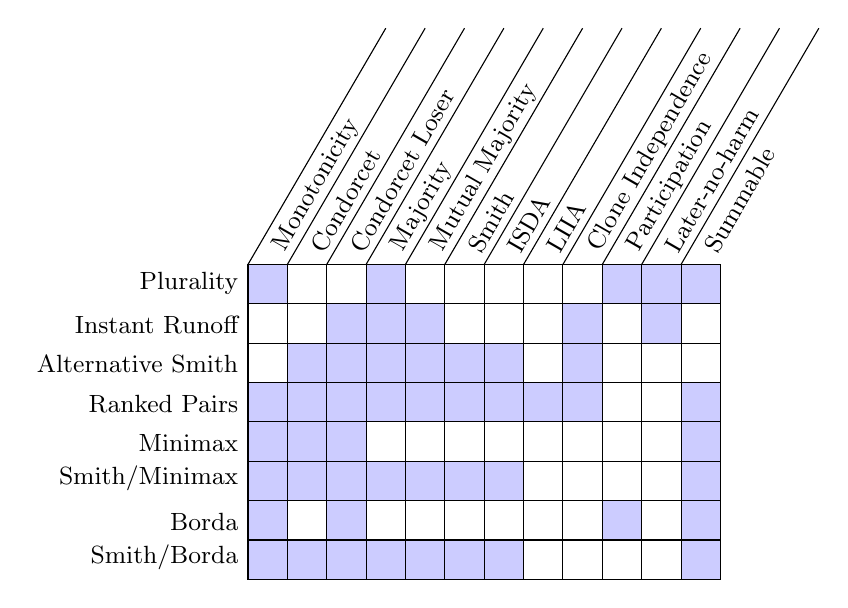
\begin{tikzpicture}[
        %sibling distance=10em,
        font=\small,
        ]
%        \foreach \x / \y in {
%            0/2,
%            1/3,
%            2/3,
%            3/4,
%            4/4,
%            5/5,
%            6/6,
%            7/7,
%            8/4,
%            9/7
%        }
%        {
%            \draw [fill=green] (\x/2,1-\y/2) rectangle ++(0.5,-0.5);
%        }
        \foreach \x / \y in {
            0/0, 3/0, 9/0, 10/0, 11/0, % Plurality
            2/1, 3/1, 4/1, 8/1, 10/1, % IRV
            1/2, 2/2, 3/2, 4/2, 5/2, 6/2, 8/2, % Alternative Smith
            0/3, 1/3, 2/3, 3/3, 4/3, 5/3, 6/3, 7/3, 8/3, 11/3, % Ranked Pairs
            0/4, 1/4, 2/4, 11/4, % Minimax
            0/5, 1/5, 2/5, 3/5, 4/5, 5/5, 6/5, 11/5, % Smith/Minimax
            0/6, 2/6, 9/6, 11/6, % Borda
            0/7, 1/7, 2/7, 3/7, 4/7, 5/7, 6/7, 11/7 % Smith/Borda
        }
        {
            \draw [fill=blue!20] (\x/2,0-\y/2) rectangle ++(0.5,-0.5);
        }
        \foreach \x[count=\xi] in {
            Monotonicity,
            Condorcet,
            Condorcet Loser,
            Majority,
            Mutual Majority,
            Smith,
            ISDA,
            LIIA,
            Clone Independence,
            Participation,
            Later-no-harm,
            Summable
        }
        {
            \node at (0.5*\xi-0.35,0) [anchor=south west] {\rotatebox{60}{\x}};
            \draw (0.5*\xi-0.5,0) -- ++(1.75,3);
            \draw (0.5*\xi-0.5,0) -- ++(0,-9/2+0.5);
        }

        \draw (0,0) -| ++(6,-4);
        \foreach \x[count=\xi] in {
            Plurality,
            Instant Runoff,
            Alternative Smith,
            Ranked Pairs,
            Minimax,
            {Smith/Minimax},
            Borda,
            Smith/Borda
        }
        {
            \node at (0,-0.5*\xi) [anchor=south east] {\x};
            \draw (0,-0.5*\xi) -- (6,-0.5*\xi);
        }

    \end{tikzpicture}
    \caption{\label{fig:single-winner-criteria}Single-winner voting rule criteria.}
\end{figure}

\begin{itemize}
    \item Begin by discussing that different voting rules—the rules about how ballots will be counted and the winner selected—have different properties affecting whose vote matters and how representative the election is.
    \begin{itemize}
        \item Recalling \hyperref[cur:majority]{the lesson on majorities}, discuss plurality versus pairwise majorities, and the behavior we've seen in instant runoff voting.
    \end{itemize}

    \item Address various criterion by examining and discussing individual rules
    \begin{itemize}
        \item Use Alternative Smith to demonstrate constriction of a voting rule to the Smith set

        \item Use Ranked Pairs and Minimax to demonstrate summability
        \begin{itemize}
            \item Summability allows us to count ballots in subsets and then add the results together

            \item Counts can be observed at the place and time of voting, maintaining integrity

            \item Counts can be added along the way, allowing continuous reporting of results as with plurality
        \end{itemize}

        \item Discuss, particularly, the perceived versus actual value of later-no-harm and participation

        \item Discuss the difference between logical failure (a rule is not mathematically immune to failing a criterion) and probable failure (a rule may fail a criterion in rare cases, or only in contrived examples)
    \end{itemize}

    \item Address primary election cycles
    \begin{itemize}
        \item With too many candidates, voters can't become informed enough to provide a sufficient number of rankings
        \begin{itemize}
            \item Many ballots don't rank the candidate who would be the Condorcet winner if all voters were as informed about all candidates as they are about their favorite \textit{and} ranked their preferences for all candidates

            \item This often results in an outcome identical to if the plurality coalition were the only voters
        \end{itemize}

        \item Discuss party primary with various rules
        \begin{itemize}
            \item Party primary excludes subsets of voters, which—as in our IRV example—allows a specific set of voters to remove choices before other voters can vote.  Compare this to serial dictatorship, where if the dictator doesn't vote, then the second dictator votes; and if the second dictator doesn't, then the third; and so forth.

            \item Plurality and Condorcet both have major flaws under party primary, due to exclusion of voters
        \end{itemize}

        \item Discuss Top-Two and Final-Five primary elections
        \begin{itemize}
            \item Both select the top several candidates with the most votes

            \item Consider ranking and Condorcet instead, removing the Condorcet winner and then identifying the new Condorcet winner until having selected enough:  with too many candidates, we can't rely on voters to rank enough to select the Condorcet winner, and you get a series of candidates all representative of a plurality group of voters

            \item Top-two can lock out the majority

            \item Final Five is less prone to majority lockout, but can be affected by vote splitting as can plurality
        \end{itemize}
    \end{itemize}

    \item Address total election cycles
    \begin{itemize}
        \item Party primary with instant runoff voting is functionally just party primary and then a vote between just the two party nominees; see Burlington, VT, 2009 Mayoral Election for three strong parties

        \item Top-Two's lock-out need not be discussed because top-two always comes down to a single pairwise election

        \item Final Five uses instant runoff as its general election; the class discussion should eventually discuss a summable Condorcet method like Ranked Pairs or Smith/Minimax
    \end{itemize}

    \item Address the Maryland House of Delegates election
    \begin{itemize}
        \item This elects multiple members

        \item Voters get one vote per Delegate to be elected

        \item Vote totals are used to elect the top 3 delegates

        \item This tends to allow a plurality of voters to control all three
    \end{itemize}
\end{itemize}

\subsection{Criteria}
\begin{todo}
    Better explanations.
\end{todo}

\begin{boxcomment}
    Do not test students on relative weakness of criterion.  This is a ridiculous thing to try to memorize and is barely useful even when doing mathematical analysis of voting rules, much less in an introductory course on philosophy and basic election mechanics.
\end{boxcomment}

\begin{definition}{Weakness}
    A voting criterion is ``weaker'' than any criterion by which it is implied.
\end{definition}

Weak criterion imply strong criterion.

\begin{itemize}
    \item Majority criterion (MC) is weaker than mutual majority (MMC) because a simple majority is also a mutual majority, and when no simple majority exists a rule satisfying MC need not elect from the mutual majority.

    \item Condorcet is weaker than mutual majority, because a Condorcet method need not elect from the mutual majority set when there is no unique Smith candidate.

    \item Mutual majority is weaker than Smith, as the Smith set is a subset of the mutual majority set.

    \item Condorcet (winner) and Condorcet loser are weaker than Smith.

    \item Local independence of irrelevant alternatives (LIIA) is weaker than IIA.

    \item Smith is weaker than independence of Smith-dominated alternatives (ISDA) because a rule electing from the Smith set may be influenced by non-Smith candidates (e.g. Nanson, Baldwin).

\end{itemize}

\begin{definition}{Independence of Irrelevant Alternatives}
    The group's preference between candidates $X$ and $Y$ is determined only by the individual preferences between $X$ and $Y$.
\end{definition}

Independence of Irrelevant Alternatives (IIA) is practically impossible to satisfy.  Approval and Score theoretically satisfy IIA if voters mark each candidate on their ballot as if they don't know of the existence of any other candidate; this is patently absurd, as whether a voter approves of a candidate or how high a score they receive is dependent on the other candidates available.

Approval reduces to plurality when candidates are diverse and match voter ideals:  voters approving only candidates roughly similar to some degree will not approve other candidates.  Broken into three or more core coalitions, the largest coalition selects the winner.  When all voters approve all but the least-liked candidate, the system is equivalent to anti-plurality.

There is no absolute measure of welfare, so the highest-scored candidate from 0 to 1 must be scored 1.0 to make logical sense.  Score's claim to IIA requires voters to not exercise full voting power; more than that, it requires an absolute scale of welfare applied correctly by all voters, by which the highest possible welfare is 1.0 and the lowest is 0.  These theoretical explanations are nonsense.

\begin{definition}{Local Independence of Irrelevant Alternatives}
    If some subset of alternatives in consecutive positions of win order is selected and all other alternatives deleted from all votes, the win order of the subset must remain unchanged.
\end{definition}

LIIA requires that if the winner is rendered unranked on all ballots, the second-place winner will win; and if the loser is rendered unranked, the second-place loser will become the last-place loser.  Few methods satisfy LIIA, notably Ranked Pairs; Kemeny-Young can become technically impossible to calculate for some candidate sets as it is NP-Hard.

Plurality fails LIIA because it simply discards all but the first rank.  Theoretically, voters have unexpressed preferences due to the ballot being single-mark.  Instant runoff voting demonstrates plurality with repeated elimination of the loser:  the plurality winner in one round is not always the plurality winner in the next.  Eliminating the plurality winner on a ranked ballot can elevate the last-place candidate above the second-place candidate.

\begin{definition}{Condorcet criterion}
    A voting rule passes the Condorcet criterion if it elects the Condorcet candidate when one exists.  Also called the Condorcet winner criterion.
\end{definition}

\begin{definition}{Condorcet loser}
    A candidate for whom every opponent receives a pairwise majority of votes.
\end{definition}

\begin{definition}{Condorcet loser criterion}
    A voting rule passes the Condorcet loser criterion if it never elects the Condorcet loser when one exists.
\end{definition}

When there is no Condorcet winner, a rule may elect anyone.  Minimax always elects the Condorcet winner, but can otherwise elect any candidate including the Condorcet loser.  All runoff methods and Smith-efficient rules satisfy Condorcet loser.

\begin{definition}{Monotonicity}
    A voting rule is monotonic if raising a candidate's ranking from its original position only increases or leaves unchanged its group ranking.
\end{definition}

Instant runoff voting fails monotonicity:  when, after running off to three options, the different votes between the Condorcet candidate and a candidate outside the mutual majority is larger than the difference between the winning candidate and a simple majority, raising the winning candidate to first place on as many ballots causes the minority candidate to be eliminated before the Condorcet candidate, and the Condorcet candidate is elected.  In this condition, ranking the winning candidate higher on several ballots causes that candidate to lose.

Many Smith-efficient methods satisfy monotonicity because raising a candidate gives them a stronger position.  Geller-IRV and Geller-STV eliminate by Borda count, and so raising a candidate decreases their likelihood of elimination while raising their likelihood of having enough votes to be elected.  Smith/IRV is non-monotonic for the same reasons as IRV.  Ranked Pairs, Schulze, Split Cycle, and others are monotonic.

\begin{definition}{Participation}
    A voting rule satisfies the participation criterion if adding a ballot where Candidate $X$ is preferred to Candidate $Y$ cannot change the winner from $X$ to $Y$.
\end{definition}

\begin{definition}{Consistency}
    A voting rule satisfies the consistency criterion if two sets of ballots tabulating to identical results also produce an identical result when tabulated together as one set of ballots.
\end{definition}

Participation and consistency reduce mathematically to the same function:  each implies the other.  No known viable voting system satisfies these criterion, notably Borda because of its extreme manipulability and plurality for obvious reasons are not considered ``viable.''

\begin{definition}{Clone independence}
    A voting rule is independent of clones when adding or removing candidates to clone sets does not affect the winning chance of any candidate not in the set of clones.
\end{definition}

We can think of a clone set as a set of candidates for which no voter ranks any candidate outside the set between or equal to those inside the set, or a rough approximation there of.  This is too broad, and in practice clones must be substantially-similar, so the definition is somewhat imprecise and conceptual.

Instant runoff voting is immune to clones because it will eliminate one or the other at the same stage, transfer votes exclusively to the surviving clone, and then place the surviving clone in the original elimination order.  Ranked Pairs is similarly immune because clones have the same (or substantially similar) pairwise victories, and so their order of placement doesn't change.  Unpopular ideological clones just end up at the bottom with few votes.

Of interest:

\begin{itemize}
    \item Smith criterion implies Condorcet and Mutual Majority.

    \item Condorcet implies Majority Winner, but does not imply Mutual Majority.

    \item Mutual Majority implies Majority Winner and Majority Loser, but not Condorcet Loser (Bucklin satisfies Mutual Majority but not Condorcet Loser).

    \item Smith is incompatible with later-no-harm, favorite betrayal, participation, and consistency, and independence of irrelevant alternatives.

    \item Any voting rule constricted to the Smith set by treating as withdrawn all non-Smith candidates is independent of Smith-dominated alternatives (ISDA); otherwise they may not be ISDA.  Nanson's and Baldwin's methods satisfy Smith, but not ISDA.
\end{itemize}

Single-winner methods and evaluation criteria
\begin{itemize}
    \item Plurality
    \begin{itemize}
        \item Satisfies
        \begin{itemize}
            \item Monotonic:  More voters voting for X can't make Y more likely to win

            \item Majority:  If there is a first-order winner, they are elected (silly criteria…)
        \end{itemize}
        \item Fails
        \begin{itemize}
            \item Clone independence:  Adding a candidate exactly as preferred by all voters as another can't change the outcome (plurality suffers vote splitting)
            \item Condorcet:  Elects the condorcet winner (Plurality doesn't even check)
            \item Majority loser:  can't elect the majority loser.  (Plurality can elect a candidate for whom a majority of voters prefers EVERY OTHER CANDIDATE over them, i.e. not just loses to everyone, but loses spectacularly)
            \item Condorcet loser:  a stronger version of Majority loser, where a candidate is preferred by some majority of voters to each other candidate, but not necessarily by a single majority to all other candidates.  (Fails this hard)
        \end{itemize}
    \end{itemize}
    \item Instant Runoff Voting
    \begin{itemize}
        \item Satisfies
        \begin{itemize}
            \item Majority:  the winner has to have a majority of votes over at least 1 other candidate (showing how useless Majority is)
            \item Mutual majority:  If a majority of voters exists whose top n preferences are the same, but in different orders, the majority with the smallest value n is the mutual majority, and the candidates in question are the mutual majority set.  The winner must be one of these.  (This paired with later-no-harm causes a severe error in IRV)
            \item …Thus Condorcet loser and Majority Loser.
            \item Later-no-harm:  if a voter ranks an additional candidate as less-preferred than all other candidates, doing so doesn't cause one of their higher-ranked candidates to lose
            \item Later-no-help:  if a voter adds a candidate as in later-no-harm, doing so doesn't cause one of their higher-ranked candidates to win.
            \item Clone independence
        \end{itemize}
        \item Fails
        \begin{itemize}
            \item Participation:  a voter can't get a better result by not voting.  (This failure is demonstrated in the first class.  Tactically, the voter is better off voting for the better result they think they will get by not voting, and their favorite second)
            \item Favorite betrayal:  a voter can't make their favorite win by ranking someone above their favorite.  (Under IRV, voting for candidate X can cause Y to be eliminated before candidate A, transferring votes to A.  This may cause A to win, whereas the same voter voting for A first can cause A to lose.)
            \item Monotonic
            \item Condorcet
        \end{itemize}
    \end{itemize}
    \item Minimax
    \begin{itemize}
        \item Satisfies
        \begin{itemize}
            \item Monotonic
            \item Condorcet
            \item Majority
            \item Summable (only need the pairwise results, so ballot counting can be divided up)
        \end{itemize}
        \item Fails
        \begin{itemize}
            \item Majority loser (implying it fails Condorcet, Mutual Majority.  Minimax can elect any candidate.)
            \item Smith:  if no Condorcet winner exists, selects from the smallest set where any single one of these would be the Condorcet winner if the others were removed.  (Failing Majority Loser, Condorcet, Mutual Majority all imply failing this)
            \item Clone independence
            \item Participation
            \item Later-no-harm/help
        \end{itemize}
    \end{itemize}

    \item Ranked Pairs
    \begin{itemize}
        \item Satisfies
        \begin{itemize}
            \item Monotonic
            \item Condorcet
            \item Majority
            \item Mutual majority
            \item Clone independence
            \item Smith
            \item Independence of smith-dominated alternatives:  candidates not in the Smith set have no effect on the outcome
            \item Local independence of irrelevant alternatives:  Deleting the last-place winner must not change the outcome; deleting the first-place winner must cause the second-place winner to be elected
            \item Summable
        \end{itemize}

        \item Fails
        \begin{itemize}
            \item Participation
            \item Later-no-harm/help
        \end{itemize}
    \end{itemize}
\end{itemize}

\subsubsection{Range Voting}

A note on range voting.

The Range Voting Web site indicates Arrow's is violated by score voting systems, but that can be proven untrue.  It's only independent of irrelevant alternatives if voters don't change their other scores, which assumes voters don't use full voting power.  Whenever a candidate is introduced who any voter prefers more than their otherwise first-choice candidate, that first-choice candidate is either scored less than the maximum (not exercising full voting power) or all scores are adjusted to fit the new top-scored candidate.  Whether other candidate scores are altered equally, unequally, or in proportion, there is a scenario where a winning candidate becomes a loser and a losing candidate becomes a winner as a result of this new losing candidate.

All Condorcet methods are independent of irrelevant alternatives when there is a Condorcet winner.  That's not the point.

\url{https://www.princeton.edu/~cuff/voting/theory.html} hits this point.

Given the possibility that any single voter may exist whose preferences are the same as their scores, with higher scores being higher preference, the conditions given to satisfy IIA cannot be satisfied.  A voter may have three candidates $\left\{A,B,C\right\}$ such as to rate $A=1.0$ and both $B=0.0$ and $C=0.0$; to elevate $C$ above $A$, the voter must reduce the ranking of $A$.  No matter how small this reduction, the margin between $A$ and $B$ can be so small as to be smaller, and so the winner changes from $A$ to $B$; and even in a finite field where movements are not infinitely small, $A$ can become tied with $B$.  This single example shows a violation of one criterion which Arrow's Impossibility Theorem says can never be simultaneously true along with non-dictatorship and Pareto.
\refstepcounter{syllabuslesson}
\label{cur:multi-winner-voting-rules}
\section{Multi-Winner Voting Rules and Elections\hyperref[syllabus]{↑}}

This lesson introduces multi-winner districts and different multi-winner rules, including single non-transferable vote (SNTV), multiple non-transferable vote (MNTV), and single transferable vote.

\begin{boxcomment}
    Dr. Uzochukwu will likely appreciate the contrast between MNTV and STV; and Prof. Willis had brought up that multi-member districts were created as a tool to suppress black voters by multiplying the majority or even plurality vote for multiple candidates, something that can be replicated under single-member districts by careful district drawing but utterly fails under STV.  (We seriously need to get rid of MNTV, and Condorcet isn't good enough for this)
\end{boxcomment}


\subsection{Assigned Reading}

\begin{itemize}
    \item Chapter 17 of the Handbook of Social Choice and Voting \autocite[303-323]{Heckelman2015}
\end{itemize}


\subsection{Overview}

Multi-winner elections:
\begin{itemize}
    \item Single non-transferable vote
    \begin{itemize}
        \item How SGA and Final Five operate
        \item Not proportional, but a bit better than MNTV
    \end{itemize}

    \item Multiple non-transferable vote
    \begin{itemize}
        \item How Maryland elects delegates
        \item Not proportional, basically plurality with bigger consequences
    \end{itemize}

    \item Serial Condorcet
    \begin{itemize}
        \item e.g. use Ranked Pairs and elect the first n-place winners
        \item Not proportional; achieves multiple representation for a given population in the way of Condorcet winners
    \end{itemize}

    \item Single transferable vote
    \begin{itemize}
        \item How New Zealand elects some multi-member districts; also Scotland and several others
        \item Proportional, due to vote transfers, breaking a population apart into like-minded voting coalitions wholly based on their votes
        \item Easy to explain Meek's Method versus other methods
    \end{itemize}

    \item Geller-STV
    \begin{itemize}
        \item Single Transferable Vote, but eliminating by lowest Borda score

        \item Has interesting properties, but isn't well-studied

        \item Geller-IRV only elects the Condorcet winner from not more than three candidates
        \begin{itemize}
            \item Geller-IRV satisfies Mutual Majority because it elects by vote count, and eventually all but one mutual majority candidate has been eliminated.

            \item Geller-IRV cannot elect the Condorcet loser for the same reason.

            \item Geller-IRV must elect the Condorcet winner between three candidates because a Condorcet winner either has a simple majority or else can only exist if two intersecting majorities of ballots rank the Condorcet winner.  As a result, the Condorcet Loser must have a lower score than the Condorcet Winner, and so the Condorcet Winner cannot be eliminated first.

            \item Geller-IRV may fail to elect the Condorcet winner with four candidates because ballots may be truncated, thus the Condorcet winner may have a lower Borda score than the Condorcet loser.

            \item By contrast, Geller-IRV tends to elect closer to the Condorcet winner when more voters tend to rank more candidates.
        \end{itemize}

    \end{itemize}

%14     A>B>C>D	A>B	    27 A>B        15 A
%12     B>A>C>D	B>A	    23 B>A        19 A>B
%25     C>B>A>D C>B>A>D 2  C>B>A>D    32 B>A
%49     D>C>B>A D>C>B>A 49 D>C>B>A    19 C>B
%                                     15 C
%
%A      91      91	    129           100
%B      163     163	    176           102
%C      199     173	    104           68
%D      147     147	    147
%El     A,D     A,D	    C,A
%Win    C       C       B
%Con    C       C       C
%IRV    B,C;A   B,C;A   B/C
%
% The third example breaks the tie between two IRV winners.
% Note in regular IRV, after C is eliminated, those voters are
% part of the {B,A} mutual majority, of which B is the Condorcet
% winner

    \item Quota Borda System
    \begin{itemize}
        \item Inherits from Borda, but looking for a quota Borda score in the same way STV looks for a quota vote count

        \item Not well-studied

        \item Complex (enough so that maybe it should be skipped here)

        \item Similar pathologies to Borda count, just as STV inherits from IRV
    \end{itemize}
\end{itemize}



\subsection{Party primary issues}

\begin{boxcomment}
    Electoral systems and government structures overlap.  I define an electoral system as a social choice process using an ordered set of elections applying social choice functions, specifically voting rules.

    Stages of electoral processes include registration, nomination, and runoffs.  The most well-known runoff in the United States is the general election following a ``primary'' nominating election.

    One possible process has several stages:
    \begin{itemize}
        \item \textbf{Registration}:  Candidates file with the election authority, satisfying legal requirements in most jurisdictions to raise and spend money.

        \item \textbf{Popular Nomination}:  Up until the registration deadline, candidates petition the public for signatures to support their candidacy.  Candidates reaching a threshold of signatures are nominated for office.

        \item \textbf{Winnowwing}:  A series of runoff elections to select
    \end{itemize}
\end{boxcomment}

\prettyref{ele:party-primary} describes an instant runoff voting failure mirrored by party primary.  This is also an argument used when dealing with FairVote's propaganda.

\begin{figure}
    \begin{election}
        \singlespacing
        \label{ele:party-primary}
        Consider the below set of 100 preferential ballots:
        \begin{itemize}
            \item 26 Alex$\succ$Bobbie$\succ$Chris$\succ$Dane
            \item 25 Bobbie$\succ$Alex$\succ$Chris$\succ$Dane
            \item 20 Chris$\succ$Dane$\succ$Bobbie$\succ$Alex
            \item 29 Dane$\succ$Chris$\succ$Bobbie$\succ$Alex
        \end{itemize}

        Pairwise, this breaks down into three elections:

        \begin{itemize}
            \item 51 Alex : 49 Chris
            \item 51 Alex : 49 Dane
            \item 74 Bobbie : 26 Alex
            \item 51 Bobbie : 49 Chris
            \item 51 Bobbie : 49 Dane
            \item 71 Chris : 29 Dane
        \end{itemize}
        Consider voters have split into groups whose top two are ${Alex,Bobbie}$ and ${Chris,Dane}$.  If we call these Parties $X$ and $Y$, respectively, then Party $X$ nominates Alex and $Y$ nominates Dane, despite a majority of voters preferring the alternate candidate in each party.  Both party primary and instant runoff voting elect Alex in this case.

        Although Bobbie is the Condorcet winner, once the party primaries remove Bobbie and Chris, Alex is the Condorcet winner among the \textit{remaining candidates}.  This can give the impression that IRV tends to elect the Condorcet winner when it is used in elections with party nominating primaries in a strong two-party system.
    \end{election}
\end{figure}

This shows similar issues to the two-tier problem:  a party excludes other voters from its nominating process; registered voters of a majority party may be considered the only voters.  Those not voting in the primary may have no preference between party candidates, although the rational calculus of voting may apply, to the point that they may have little enough preference to rank them in a general election but not to bother voting in a party primary.

When a party of 51\% of voters nominates the far extreme by 51\% of the party, the general election elects by 51\% of 51\% or 26.01\%.  Assuming all party electees are elected by like-minded voters, a Senate of 100 Senators of equal-sized districts is controlled by 51\% of that, or 13\%.

There are two problems with this analysis.

First, party voters are not like-minded, and have regional differences.  That 51\% is not one mind.  Second, U.S. Senate districts are not of equal size, so less-populus States in the 51\% may represent less than 10\% of voters in the Senate.

Tideman, Green-Armytage, myself, and others have converged to Single Transferable Vote primary elections to nominate for a Condorcet general election.

We have differences in opinions, e.g. Tideman and others suggest a modified STV to protect the Condorcet candidate from elimination, while I don't believe there's enough information to \textit{find} the Condorcet candidate.  In a practical sense, voters will have diverse opinions between 60 different options—we have seen this in a Delegate election by MNTV in District 40, with 20 candidates and 15 of them all had more than 10\% of the vote, and the highest vote count was barely over 20\%.  They won't rank more than 5 or 6, usually, and may not even understand them all due to the economics of investing time in learning about candidates.  The Condorcet candidate among the biggest coalition will be recognized as the Condorcet candidate among all voters, mathematically, due to low information.

I favor Ranked Pairs; so did Tideman, until someone convinced him Minimax was about as good and simpler to understand.  I disagree:  describing Ranked Pairs is more engaging, and requires explaining each candidate's greatest win margin; Minimax requires explaining that for \textit{all} of each candidate's loss margins, we find the \textit{biggest} one, and then find the candidate who has the \textit{smallest} one of that.  Minimax can fail and elect the Condorcet loser when there is no Condorcet winner, so then you have to explain the Condorcet winner and the Smith Set as with Ranked Pairs, and restrict to the Smith Set.

Mostly we're on the same page.

Katherine Gehl prefers Final Five, which uses Single Non-transferable Vote to nominate five, then Instant Runoff Voting to elect one.  Japan's experience with SNTV was not great.  Instant Runoff Voting isn't summable and is considerably broken.  Gehl's explanation is that explaining voting systems is hard, and IRV and top-n (SNTV) are already popular and well-known—the lack of public understanding of social choice theory and voting theory is the impetus for this course, and this is a consequence of a lack of adequate public education.

\begin{todo}
    References for Japan:

    G.W. Cox, F.M. Rosenbluth
    Factional competition for the party endorsement: the case of Japan's Liberal Democratic Party
    British Journal of Political Science, 26 (2) (1996), pp. 259-270

    G.W. Cox, F.M. Rosenbluth
    Electoral rules, career ambitions, and party structure: comparing factions in Japan's upper and lower houses
    American Journal of Political Science, 44 (1) (2000), pp. 115-123

    G.W. Cox, F.M. Rosenbluth, M.F. Thies
    Electoral reform and the fate of factions: the case of Japan's Liberal Democratic Party
    British Journal of Political Science, 29 (1) (1999), pp. 33-50

    S. Reed
    Strategic voting in the 1996 Japanese general election
    Comparative Political Studies, 32 (2) (1999), p. 257

    Japan: Manipulating Multi-Member Districts — from SNTV to a Mixed System
    DOI 10.1057/9780230522749\_30

    Manipulating Electoral Rules to Manufacture Single-Party Dominance
    Kenneth Mori McElwain
    American Journal of Political Science
    Vol. 52, No. 1 (Jan., 2008), pp. 32-47 (16 pages)
    Published By: Midwest Political Science Association
\end{todo}

That single-party dominance can be established by manipulating SNTV is troubling.  I must research this further.
\refstepcounter{syllabuslesson}
\label{cur:government-structure}
\section{Government Structure\hyperref[syllabus]{↑}}

Brings this all together with government structures.  This lesson addresses topics like k-majorities and the US Senate filibuster, single- versus multi-member districts, and City governments.

The case study used for Maryland State government retains the structure of government but alters the voting rules to engineer something completely different in its basic design.  This demonstrates a diversity of voices from each district in the House of Delegates, and a consensus of each district in the Senate, and in the Executive.

The case study for Baltimore City \textit{completely} re-engineers the government, and the merits of elected versus appointed executives should be compared more carefully to not evagicalize a proposed government structure.  That structure is one I actually proposed in a modification of the NCL's Model City Charter.  There are interesting interactions and implications for the Council body, and I tailored the specific details to distribute the ``power of corruption'' to increase the amount of collusion required to pull off what an elected Mayor can do in backroom deals, making such collusion dangerous, hard to keep secret, and unstable across elections.  It's not just ``we need our votes to count,'' but a whole examination of what the government structure accomplishes and how the method of voting and representation affects that.

\begin{boxcomment}
    Supermajority rule and bicameral legislatures have a similar effect to k-majority rule in making the vote more demanding and reducing the number of possible values to fit greater consensus \autocite[180]{Heckelman2015}.  The U.S. Senate has unique powers in approving treaties and executive appointmetns, notably including Supreme Court Justices; becaus this circumvents the decision-making complexity of a bicameral legislature, k-majortiy has large democratic merits.  This is hotly debated today; if you want to convince the students of this, you'll have to give them the tools to reach the same conclusion—pry at them to make sure they're not simply letting you dictate what they should think.
\end{boxcomment}

\begin{boxcomment}
    See ``The Misguided Renaissance of Social Choice'' by Maxwell L. Stearns, arguing that Madison and Jefferson never read anything by Condorcet about the Condorcet paradox or unicameral legislatures.  Interesting, but not addressed.

    This piece has an interesting examination of normative proposals; two quotes stand out:

    ``Scholars have used Arrow's Theorem to argue that legislative bodies are fundamentally incompetent, justifying significantly expanded judicial review.''

    Jeremy Waldron would have an aneurysm.

    ``Frank Easterbrook and others, for example, have observed that appellate courts, including the Supreme Court, are collective decisionmakers subject to the tenets of social choice.  This insight undermines arguments for expanded judicial review that are premised on the ground that legislatures are uniquely susceptible of cycling.''

    This is not necessarily true.  The Justices, as with the legislators, are a voting collectivity.  Legislators are elected in a process exposed to cycling; they are also prone to cycling, but usually get binary choices.  Recognizing considerations of social choice is not inconsistent particularly because of k-majority impacts on decision versus outcome costs, and there is a particularly strong argument for requiring a supermajority of Justices to make a Supreme Court decision.
\end{boxcomment}

\begin{boxcomment}
    Fun fact:  Nevada has a unicameral legislature.  Studying its performance is an extremely complicated matter requiring heavy statistical analysis and all kinds of skills you'd probably only learn in graduate school.  This course would prepare students to understand the resulting research, but not to carry it out themselves.
\end{boxcomment}

\subsection{Overview}

\begin{itemize}
    \item Bicameral legislature
    \begin{itemize}
        \item Condorcet argued that unicameral legislature was more efficient than bicameral and that bicameral gained nothing (Possibly move to the history lesson?)

        \item Bicameral legislature increase the complexity of decision making, similar to k-majority rules with $k>50$.

        \item U.S. Senate has unicameral confirmation of treaties and Executive appointments.
        \begin{itemize}
            \item Consider the historical margins for confirming Supreme Court Justices versus the recent 50+1 rules

            \item This is a good time to revisit the two-tier issue, considering the Senate's dissimilar-sized districts (States) with equal numbers of Senators
        \end{itemize}
    \end{itemize}

    \item Alternative construction:  Maryland State Government
    \begin{itemize}
        \item House and Senate are currently single-district, one Senator, three Delegates by MNTV, all 4-year non-staggered terms

        \item One proposal has been dividing Senate districts into three Delegate districts, rather than one multi-member Delegate district
        \begin{itemize}
            \item Arguments against multi-member districts have focused on racist motives to minimize minority votes

            \item Impact of various electoral methods, e.g. plurality, Final Five, STV nominating primary with Condorcet election

            \item Maximum representation means each Delegate is a geographical median voter, each Senator is the geographical median voter from three Delegate districts
        \end{itemize}

        \item Another proposal has been STV for Delegates\footnote{Eric Luedtke once brought this up in a private conversation.}
        \begin{itemize}
            \item Discuss prior argument about multi-member districts

            \item Compare MNTV with STV in multi-member districts

            \item Students should discuss the merits of Condorcet single-member Delegate districts versus STV multi-member Delegate districts

            \item The effects of gerrymandering are significantly different between these two
        \end{itemize}

        \item Bringing it all together:  engineering a government with heavy consideration of the voting rules.  Cajole students into exploring how voting rules can be leveraged as such.
        \begin{itemize}
            \item Condorcet Governor and Senators, STV multi-member Delegates

            \item The bicameral legislature creates complexity to improve the quality of legislation

            \item The Senate is a moderating voice, representing the diversity of views of Marylanders geographically, but within those geographic delineation represent consensus

            \item The House represents the greater diversity of views of Marylanders, not ony geographically but within geographies, creating contention and leading thought by elevating minority voices further than a Condorcet system can

            \item Compare 4-year House/Senate terms with 2-year Delegate, 4-year Senator terms as in most States; staggared Senate elections; and 4-4-2 staggering as in states such as Deleware

            \item Avoid raising questions of successorship unless the students raise them; see Baltimore City case study regarding five at-large members
        \end{itemize}
    \end{itemize}

    \item Alternate construction:  Baltimore City Government
    \begin{itemize}
        \item Current City government is elected strong-mayor with a unicameral legislature, 14 wards of 45,000 population plus one at-large City Council President, and four-year terms for all

        \item Proposition:  ten wards, five at-large by STV, City Council President selected by City Council from its five at-large members
        \begin{itemize}
            \item Ward size is comparable to Baltimore County

            \item Contrast five at-large by STV with Condorcet in 14 wards and a Condorcet Council President

            \item Contrast 15 wards with a supermajority- or Condorcet-elected Council President elected from and by the Council body with the proposed five at-large and Council President elected exclusively from those

            \item Consider backfilling a vacancy in the five at-large members.  There are several common methods
            \begin{itemize}
                \item Callback:  protect all remaining members as elected, withdraw the vacating member, and recompute the STV election without them (this may be more sensible with Geller-STV, but you have to automatically assume quota if you're recalculating Borda scores from fractional vote transfers).  Note STV can change all members, and so just rerunning it can return a bunch of candidates who may not represent those voters whose candidate vacated, hence the protection of these candidates.

                \item Special election:  Can only really be Condorcet.

                \item Successorship:  Vacating member nominates a successor; or multiple successors for either a special election or appointment by the body of City Council, or by some kind of Appointment Committee.  Informally request the member nominate at least one viable callback candidate.

                \item Appointment:  Successorship but the member doesn't have any formal privilege in determining who is appointed.

                \item Stall:  if close to the end of the session or the end of the term, do nothing.  Use two-year terms for the at-large members.  May combine well with callback or successorship.
            \end{itemize}
        \end{itemize}

        \item Proposition:  Council-manager structure in the 10/5 proposition above
        \begin{itemize}
            \item Democratic legitimacy of City manager appointed by City Council
            \begin{itemize}
                \item City Council is elected by voters, and the voters must also approve a Charter giving Council the power to appoint the Executive

                \item City Manager may be more aligned to Council and so better execute as part of a functional government; but see the two-tier problem
            \end{itemize}

            \item Does the voting rule Council uses matter?  Is Condorcet necessary, or only supermajority?
            \begin{itemize}
                \item A Condorcet rule is complicated, but creates an all-majorities intersection protecting against $k=50$ simple majority rule

                \item A supermajority rule pays some regard to the two-tier a-priori voting power problem, but makes it more difficult to \textit{remove} the City Manager

                \item Caveats on removal:  in theory, only a few members need to switch positions to remove the City Manager—more with $k>50$.  In practice, people become less apt to change the outcome once it is in place for a little while.
            \end{itemize}

            \item ``Power of corruption''?
            \begin{itemize}
                \item An elected Executive can act more freely, without accountability to City Council, and so cannot be removed for corruption if the evidence doesn't reach a legal threshold

                \item An appointed Executive can be removed by a vote of Council members, and so the ``power of corruption'' is distributed such that Council members must be colluding \textit{or} the corrupt behavior must create no suspicion

                \item Corruption becomes harder to hide the more of it an official carries out, but this becomes more obvious to Council than to voters (compare recall elections of an elected mayor and debate whether Council would respond \textit{correctly} or at least to little harm, \textit{more reliably}, and \textit{more quickly} to corruption)

                \item Corruption is harder to hide \textit{when there are more co-conspirators}
            \end{itemize}
        \end{itemize}
    \end{itemize}
\end{itemize}

\begin{boxcomment}
    I examine STV vacancies in the City government model because the five elected candidates are more diverse than when electing three.  This is an interesting consideration:  when electing more winners, appointing or electing at-large to fill a vacant seat disenfranchises fewer voters (by selecting a candidate not well-aligned to them), but excludes their voice to a much greater degree than when electing fewer winners.  At the same time, other winning candidates are ideologically closer, diminishing the degree of exclusion, but not eliminating it.

    With an odd number of candidates, one should be approximately the Condorcet candidate (STV-B might make this highly-likely, but can't identify which is the Condorcet candidate); in any case, candidates become more dissimilar in pairs, as per Plott's Majority Rule Equilibrium Theorem and Plott symmetry.  Replacing the furthest-out candidates with a Condorcet winner has obvious implications.
\end{boxcomment}
\refstepcounter{syllabuslesson}
\label{cur:evaluating-decision-methods}
\section{Evaluating Decision Methods\hyperref[syllabus]{↑}}

Discusses criteria for evaluating collective decision procedures.  Are they efficient?  Equitable?  Stable?  This covers outcome efficiency, which determines if there is a consensus or if the system doesn't reflect the voters.

This builds directly on Tideman's taxonomy of decision making methods.  There is a small bit of conceptual consideration which raises enormous, unending questions and the entire class will be high-quality debate.  That voting can cause inequality and unjust results due to the tyranny of the majority runs up against the Condorcet winner being selected by all majorities, and the median voter.

I still want to examine this for more content and really need to dig into this week's lesson.

\subsection{Assigned Reading}

\begin{todo}
    Put together a complete reading summarizing Tideman's explanations.
\end{todo}

\begin{boxcomment}
    This stuff is based on chapters 4-5 of Collective Decisions and Voting \autocite[35-56]{Tideman2006}.  I was going to summarize in \prettyref{apx:evaluating-dm}, but the ebook is available via interlibrary loan for free.
\end{boxcomment}

\begin{itemize}
    \item Collective Decisions and Voting, chapters 4 and 5 \autocite[34-56]{Tideman2006} or a substitute reading
\end{itemize}

\subsection{Overview}

This is seriously just a three-hour philosophical discussion.  There's nothing to teach here; the concepts presented by Tideman tie into everything already taught, and we can debate the various forms of efficiency, equity, and stability against concepts of ethics and constitutional consent for literally centuries.

Occasionally, someone injects into a conversation that "more democracy is always better," which may become relevant here.
\refstepcounter{syllabuslesson}
\label{cur:manipulation}
\section{Electoral Manipulation\hyperref[syllabus]{↑}}

\begin{boxcomment}
    It's disconnected from the rest, except insomuch as its logical relationship building on modes of collective decision and on the flaws that prevent voting from producing good outcomes and high equity, as well as to the concepts of representative democracy, government structure, and general democratic legitimacy which are predicated on voting actually being democratic.
\end{boxcomment}

Covers strategic voting, then strategic nomination.  This is where I weaponize the flaws in various systems.

Strategic voting picks up from the Score Voting discussion, and brings up Approval voting as a scored system in which all scores are 1 or 0.  The propensity of voters to vote strategically when the utility of strategy increases is a direct point of focus, both for democratic legitimacy reasons and for the concern of whether the system is fair to voters.

In plurality, voting for your favorite candidate always helps them win; however, this can cause your second favorite to lose when your favorite loses.  This is also true of instant runoff voting, as demonstrated in week 1.  Score systems exhibit similar:  because scores are always distributed, expressing any preference or admitting the approval of or any utility of a candidate helps that candidate defeat the voter's preferred candidates.  This puts voters under pressure, especially in close elections by approval or score:  by voting honestly, they are highly likely to elect a less-favored candidate when their favorite could win; yet by voting tactically, they may be able to win by majority, and if not then they may lose their vote entirely and only earn an even-less-favored candidate.  The closer an election, the more risk a voter faces when deciding whether or not to rate or approve a candidate.

Condorcet systems suffer these failures when there is no Condorcet winner; and it is difficult in practice to use tactical voting to control the outcome, as it requires immense knowledge of all votes cast and control over a significant portion of the ballots.

More interesting is strategic nomination.  As with tactical voting in score and approval rules, strategic nomination is exploited immediately in vulnerable systems.  Kiribati is a good example with the Borda count \autocite{Reilly2002}.  Strategic vote-splitting can affect IRV or plurality when used by candidates who understand the demographics sufficiently well.

Candidates also manipulate the election by strategic campaigning.  In Maryland, candidates for Delegate will run on slates, allowing them to effectively pool votes.  Voters who like one candidate will often vote for the others endorsed by their favorite; a large enough group of voters dominates all others, and the whole slate is elected.  Similarly, candidates campaign in a party primary to cater only to the party voters they believe they need to win; they then campaign to attract swing voters, typically a more moderate stance.

\subsection{Assigned Reading}

\begin{todo}
    Cite fun things like the government and a political party immediately hacking Borda count \autocite{Reilly2002} by strategic nomination to eliminate a popular opposition candidate.
\end{todo}

\subsection{Overview}

\begin{todo}
    Cover manipulating flaws in various elections.  This includes runnign to the party/running to the center in a party primary system; vote-splitting attacks on a general election or on a top-two primary; and slates in MNTV as used by Maryland for Delegate elections.

    This is an apt place to describe the absolute hell that is Group Voting Ticket, where voters mark a party on their ballot and the party gets one ballot to fill out however they please for each voter doing so.  This allows parties to mathematically analyze the election and manipulate the outcome, as they have a large amount of knowledge about ballots as cast.  GVT is the ultimate form of tyranny feeding on ignorance.
\end{todo}
\begin{itemize}
    \item Borda Count in Kiribati, using the highly-vulnerable Nairu method, was manipulated immeditaely.  It's a good case study as an opener, showing strategic nomination and strategic voting.

    \item Robbie Robbinette's research on strategic campaigning to bracket strong candidates out of elections via instant runofff voting displays another avenue, based on the demographics knowledge of candidates and campaign managers.

    \item Tactical voting is the weakest
    \begin{itemize}
        \item Tactical or ``sophisticated'' voting (sometimes called ``strategic'') is only successful when the voters obtain a benefit; vulnerability can be considered in how many votes must be altered, how much of a change can be made (e.g. how far from the Condorcet candidate can you move with how much difficulty), and likelihood of negative effects (is there real risk of electing a worse candidate instead of one the strategic voter likes more?)

        \item Discuss in general the large amount of knowledge of other voters's votes required to manipulate resistant systems.

        \item Group Voting Ticket (GVT):  largely eliminated, Australia used to use it.  Voters assign their ballot to a party, which can then file that number of ballots—giving a huge amount of precise knowledge regarding many ballots, and the ability to manipulate them at will.  GVT is concentrated evil.

        \item Again, instant runoff voting is vulnerable to strategic nomination; but it is highly resistant to tactical voting.
        \item Some systems are particularly vulnerable nonetheless, e.g. Borda, especially Nairu (tournament count is less vulnerable).

        \item IRV is resistant primarily because every round of elimination is done without regard to further rankings, which creates a large cost.

        \item Some systems force strategy:  score and approval voting help every candidate rated or approved, and in a close election this means voting honestly can turn a favored winner into a loser.  Ranked systems can fail in that way, but typically are more monotonic even when they are mathematically capable of failing in that way in certain situations.
    \end{itemize}

    \item A voting rule cannot be made more vulnerable by adding a Condorcet restriction, but can be made less vulnerable.
    \begin{itemize}
        \item Condorcet-Hare systems tend to be highly resistant to manipulation

        \item Black's method (if there is a Condorcet winner then elect them, otherwise use Borda) or Smith-constrained Borda are much more resistant to strategy than Borda.
    \end{itemize}

    \item Elections can be manipulated by controlling the options
    \begin{itemize}
        \item Referendum where four options have a majority
    \end{itemize}

    \item Not all rules are well-researched
    \begin{itemize}
        \item Single Transferable Vote is immensely strategy-resistant; STV-B and Meek-Geller are much less researched, but may be resistant due to eliminating by weakness of Borda score but electing by strength of votes.

        \item Black's is well-known, but Smith/Borda is not; although all Smith candidates generally have the same legitimacy

    \end{itemize}

\end{itemize}

\subsection{Particular Attacks}

These attacks can be discussed in class as examples.  The instructor should be familiar with these systems and the various methods of manipulation.

Tactical voting I usually consider infeasible, but it has a place in score systems and in Borda; Group Voting Ticket—where a voter checks a party and deposits their ballot, and that number of ballots are given to the party to fill out as they see fit—is the most concentrated evil, giving essentially one voter (an administrative entity) an enormous amount of knowledge about many votes because that voter is allowed to cast them.  Where GVT or straight-party ticket is used, these options are selected as high as 90\% of the time, which underscores how dangerous and destructive these are.

\subsubsection{Binary Votes}

Binary votes, such as are used in legislatures, can be easily manipulated.  Within legislatures, the best solution is k-majority with $k>50$.

Consider the ballots in \prettyref{ele:pr-ref}.  Statehood is the Condorcet option; there is a cycle from Independence to Status Quo to Commonwealth.  The authority creating the ballot referendum can dictate the outcome by selecting any of these, for example by asking if Puerto Rico should become a Commonwealth or stay as is, the voters will vote Commonwealth; asking to decide between Commonwealth or Independence will select Independence.  This is most effective by pitching a Commonwealth as a greater stage of self-governence, as if it were a natural middle ground from the status quo, or effectively no change when placed next to Independence.

\begin{figure}[ht]
    \begin{election}
        \label{ele:pr-ref}
        Referendum on Puerto Rican Statehood

        \begin{itemize}
            \item 40: Statehood$\succ$Independence$\succ$Status Quo$\succ$Commonwealth
            \item 35: Commonwealth$\succ$Independence$\succ$Statehood$\succ$Status Quo
            \item 15: Status Quo$\succ$Statehood$\succ$Commonwealth$\succ$Independence
            \item 10: Status Quo$\succ$Commonwealth$\succ$Independence$\succ$Statehood
        \end{itemize}
    \end{election}
\end{figure}

These ballots would produce a 75\% vote for Statehood using the question proposed in the real-life referendum, ``Should Puerto Rico be immediately admitted into the Union as a State?''  At the same time, it would receive a 75\% vote for Independence using the question, ``Should Puerto Rico be immediately recognized as an independent nation?''

Despite the landslide vote for Independence, the question, ``Should Puerto Rico be recognized as a State of the Union or as an independent nation?'' would result in a 55\% vote for Statehood.  Likewise, asking only if Puerto Rico should become a Commonwealth would, assuming the above ballots, select the Status Quo.

Only the last one would be readily recognized as a false choice.  A vote for Independence, without a vote for Statehood, would be assumed as a great shift in voter sentiment away from Statehood to an independent Puerto Rican nation.  A vote between Commonwealth and Independence may be interpreted as Puerto Ricans preferring the Status Quo and voting to build upon it with the move to a Commonwealth, despite Puerto Ricans opposing moving from Status Quo to Commonwealth.  This provides a great opportunity for propaganda from an election authority willing to manipulate the referendum by controlling the options on offer.

In the example given, a 60\% supermajority vote would fail when voting for Statehood against Independence; while a 70\% supermajority vote would succeed when voting for Independence against the Status Quo.  This, as well, can be used to convince voters they really voted for Independence, so long as the vote between Statehood and Status Quo isn't presented for a vote:  voters will raise questions when both Statehood and Independence achieve a 70\% supermajority over Status Quo, but Independence is selected because only a 55\% simple majority select for Independence over Statehood.

k-majority with $k>50$ works for legislation because bills are complex and legislators must negotiate over the details until the bill is acceptable to a supermajority body.  Legislation is always a complex question, although it can be considered as a variety of possible bills passing a supermajority, which can be placed into the framework of a Condorcet vote.

\subsubsection{Plurality and MNTV}

Everybody already knows plurality is easily manipulated by vote splitting.  Technically, this is done by running clones.

Multiple Nontransferable Vote, used in Maryland's Delegate elections, is usually attacked by using a slate.  Each candidate associates themselves with another candidate on the slate, effectively pooling votes.  Candidates who appeal to different demographics draw in different voters by the virtue of being roughly similar and vouching for each other's similarity.

MNTV can also be attacked by vote splitting, like plurality.

\subsubsection{Instant Runoff Voting and Single Transferable Vote}

Already demonstrated strategic nomination on Day 1.

Robbie Robinette gave a presentation on forcing IRV to fail by campaign strategy, which exploits the same flaw.

Single Transferable Vote is much more difficult to manipulate.  The flaw in IRV is contained to a narrower scope because of quotas and partial transfers of voting power.

STV provides a chance of Woodall free riding, where a voter ranks an unpopular candidate first and their favorite second, hoping that other voters will elect their favorite in the first round and they will avoid a partial transfer, keeping their whole vote.  Meek's STV avoids this by computing the winners as if all eliminated candidates were eliminated before all elected candidates.  Meek's can protect agaist Hylland free riding, where a voter simply doesn't rank their favorite at all; Hylland carries more risk, as the candidate can more easily become unable to win.

STV-B, or Geller-STV \autocite{Geller2005}, may provide better representation under STV.  Reduced to one winner at a $\nicefrac{1}{2}$ quota, or IRV-B, it shows resistance to tactical voting and strategic nomination.  This requires more research; two propositions show promise:

\begin{itemize}
    \item Eliminating a candidate earlier requires lowering them on the ballot, which means they are more likely to lose if a higher-ranked candidate on that ballot loses, making the outcome worse for the voter voting tactically

    \item Higher-borda-score candidates will appear more often higher-ranked, so eliminating the winning candidate is either difficult because the original first loser is already low

    \item Because of STV's severe strategic consequences for not ranking sufficient candidates, despite little if any advantage to ranking much more than $\nicefrac{n}{s}$ candidates for $n$ candidates and $s$ seats to elect, voters will maximize their vote by voting similarly under Geller-STV as they do under e.g. Meek-STV.

    \item Voting similarly to other STV methods under Geller-STV should approach a generalization of Geller-IRV's convergence toward a Condorcet result.
\end{itemize}

Failures seem to elect the IRV winner when there is no Condorcet winner, similar to Smith/IRV.  This rule has not been studied enough, and it is not documented if this elects from the Smith set; it cannot be independent of Smith-dominated alternatives.

IRV-B must satisfy mutual majority, as election is by vote count, and so the last candidate in the mutual majority set cannot be eliminated prior to election.

IRV-B satisfies Condorcet Loser, as the Condorcet winner must have a higher Borda score than the Condorcet loser\footnote{Elizabeth Patitsas, 2007, Can the Borda Count ever rank the Condorcet loser ahead of the Condorcet winner?}.

%It satisfies the Condorcet criteria because the Condorcet candidate must be in the mutual majority, the Condorcet candidate must have a majority vote count over others in the mutual majority, and the Condorcet candidate must gain more Borda count from outside the mutual majority than non-Condorcet candidates.  That is:  the Condorcet candidate must have the highest Borda count of the mutual majority candidates, but not necessarily the highest Borda count.

%49 A>B>C>D  A=149 B=150 C=197 D=98
%1 B>A>C>D
%49 C>X>Y>Z>D>B>A  A=299 B=300 C=494
%
%49 A>B>C>D  A=149 B=150 C=197 D=98
%49 B>A>C>D
%1 C>X>Y>Z>D>B>A  A=299 B=300 C=686

% Satisfies participation?  Not voting lowers the vote count for a higher candidate; voting raises the borda count for a higher candidate more than a lower candidate.

%\begin{table}
%    \begin{tabular}{|c|c|c|}
%        \hline
%        Count & Ballots & Borda Score \\
%        \hline
%        35 & $A\succ B\succ C$ & $A = 102$
%        \hline
%        32 & $B\succ A\succ C$ & $B = 132$
%        \hline
%        33 & $C\succ B\succ A$ & $C = 66$
%        \hline
%    \end{tabular}
%    \caption{IRV elects A; IRV-B eliminates C, elects B.}
%\end{table}
%
%\begin{table}
%    \begin{tabular}{|c|c|c|}
%        \hline
%        Count & Ballots & Borda Score \\
%        \hline
%        35 & $A\succ C\succ B$ & $A = 102$ \\
%        \hline
%        32 & $B\succ A\succ C$ & $B = 97$ \\
%        \hline
%        33 & $C\succ B\succ A$ & $C = 101$ \\
%        \hline
%    \end{tabular}
%    \caption{After tactical voting, IRV elects A; IRV-B eliminates B, elects A.}
%\end{table}
%
%The third election shows risk.  If one voter shifts from the $A$ set to the $B$ set, the tactical manipulation elects $C$.  Both manipulations fail unless almost all $A$ voters raise $C$ above $B$.
%
%\begin{table}
%    \begin{tabular}{|c|c|c|}
%        \hline
%        Count & Ballots & Borda Score \\
%        \hline
%        34 & $A\succ C\succ B$ & $A = 100$ \\
%        \hline
%        33 & $B\succ A\succ C$ & $B = 99$ \\
%        \hline
%        33 & $C\succ B\succ A$ & $C = 101$ \\
%        \hline
%    \end{tabular}
%    \caption{Risk in tactical voting.}
%\end{table}

\subsubsection{Borda Count}

Borda Count has an interesting property:  it may not elect the majority winner or the Condorcet winner.  Wikipedia has an example where Catherine is basically every voter's second choice and only a few voters's first choice; Andrew is the first choice of 51\% of voters; but Andrew is the \textit{last} choice of 49\% of voters.  This works for three candidates:  Borda elects Catherine.

The obvious attack, when Andrew is expected to have a high Borda score, is to place Andrew at the bottom.  If the 49 voters prefer Andrew second and Andrew is moved from second to last place, Andrew becomes the loser.  This has a simple hazard:  there are all of four candidates, and the common second-place winner ends up winning unless this second-place winner is the last choice of Andrew voters, in this case David.  As with all strategic voting, this requires advanced knowledge of the opposite voting coalition.

In practice, this manipulation is dangerous, but damaging even when unsuccessful.  Elevating Donald Trump, for example, makes Trump a much more likely electee.  This can be combined with a second attack:  strategic nomination.

With Borda, under the Dowdall or ``Nauru'' system, each candidate at rank $n$ receives $\frac{1}{n}$ points.  In the more common tournament-style ranking, which is much less manipulable, for an election between $c$ candidates, each candidate at rank $n$ receives $c-n$ points, e.g. when there are five candidates, the top-ranked receives $5-1=4$ points, and the last receives $5-5=0$ points.

With four candidates, a first-place candidate Alex on 51 ballots ranked last on 49 receives $3\times51=153$ points, and a candidate Bobbie ranked in second place on 49 and last on 51 ballots will receive $2\times49=98$ points or 64\% as many.  With eight candidates, these figures are $7\times51=357$ and $6\times49=294$, 83\% as many.  Borda count is heavily influenced by the presence of irrelevant alternatives.

Adding non-running candidates and last-ranking the majority winner gives no points on those ballots last-ranking this winner, but brings the losers closer.  Consider if 27 ballots ranked Alex first and Bobbie second, and 49 ranked Bobbie second and Alex last.  With four candidates, this gives Bobbie $2\times76=152$ points.  With eight candidates, these figures are $7\times51=357$ for Alex and $6\times76=456$ for Bobbie:  the existence of irrelevant candidates elevates Bobbie to victory even if the first four rankings on every ballot are the same, except that Alex is moved to stay last on 49 ballots.  However, if Alex stays in fourth place, the total adds $4\times49=196$ for a total of 553; therefor this attack relies on the knowledge that voters will rank Alex last if given more options.

There are a few possible defenses:

\begin{itemize}
    \item Restrict to the Smith set

    \item Restrict to some number $c$ of candidates based on some criteria
\end{itemize}

Restricting to the Smith set makes the rule independent of Smith-dominated alternatives, and a Condorcet rule.  This has some merit, as seen in the ability of Borda to elect despite a majority preference:  it may select a better welfare candidate.  Manipulation is likely to be filtered out in Smith/Borda, but this is not a mathematical guarantee; on the other hand, its outcome can be no worse than any Smith-efficient method.

Restricting to some number $c$ of candidates is more complex.  Using the top $c$ candidates ranked in the top $n$ ranks would tend to favor a plurality or majority coalition, for example a majority party.  Using the top $c$ borda scores may be more feasible.

None of these is summable:  that a candidate appears at a particular rank or has a particular score does not reveal anything about the candidate's relative position versus any other candidate on any ballot.  Smith/Borda can be summed by not recalculating the Borda score, but this defeats much of the purpose.  All possible calculations can be computed, but this is not more compact than the ballots themselves.  Putting summability aside, either of these greatly restricts the strategic manipulability of the Borda count.

\subsubsection{Quota Borda System}

Quota Borda System is more reliable than Borda, but still relies on Borda scores and can be manipulated in the same way.  These manipulations elevate all higher-ranked candidates, so have less of an impact.

QBS has some complexity and several pathologies.  Unlike Borda, the number of points awarded depends on how many candidates are ranked, which encourages voters to rank candidates between which they don't really differentiate—awarding points to candidates for whom the voter intends to award zero points, because to award zero points the voter must sacrifice points for their favorite.

QBS doesn't provide much of an advantage because it's not summable.
\refstepcounter{syllabuslesson}
\label{cur:propaganda}
\section{Investigating Propaganda}

This lesson investigates propaganda from FairVote, Center for Election Science, and Center for Range Voting.  Students should be prepared to identify not only problems with the proposed systems, but inconsistent and deceptive statements.
}